\documentclass[article]{elsarticle}

\usepackage{lineno,hyperref}
\usepackage{amsfonts,amssymb}
\usepackage{mathtools}
%\usepackage{mathbbol}
\usepackage{bbm}
\usepackage{multirow,algorithm2e}%
\usepackage{xargs}

\newcommandx{\CPE}[3][1=]{{\mathsf E}_{#1}\left[\left. #2 \, \right| #3 \right]}
\usepackage[textsize=footnotesize]{todonotes} % pour voir les commentaires

\newcommand{\eric}[1]{\todo[color=purple!10, author=Eric]{#1}}
\newcommand{\erici}[1]{\todo[inline,color=purple!10, author=Eric]{#1}}
\newcommand{\denis}[1]{\todo[color=green!10, author=Eric]{#1}}
\newcommand{\denisi}[1]{\todo[inline,color=green!10, author=Eric]{#1}}

\def\rmd{\mathrm{d}}
\def\rme{\mathrm{e}}
\def\rset{\mathbb{R}}
\def\NtrainPath{T}
\def\TrainSet{\mathcal{T}}
\newcommandx{\EstFunc}[3][1=N]{\bar{Q}^{#1}_{#2,#3}}
\newcommandx{\EstFuncSmp}[3][1=N]{\widehat{Q}^{#1}_{#2,#3}}
\modulolinenumbers[5]

\journal{Journal of \LaTeX\ Templates}

%%%%%%%%%%%%%%%%%%%%%%%
%% Elsevier bibliography styles
%%%%%%%%%%%%%%%%%%%%%%%
%% To change the style, put a % in front of the second line of the current style and
%% remove the % from the second line of the style you would like to use.
%%%%%%%%%%%%%%%%%%%%%%%

%% Numbered
%\bibliographystyle{model1-num-names}

%% Numbered without titles
%\bibliographystyle{model1a-num-names}

%% Harvard
%\bibliographystyle{model2-names.bst}\biboptions{authoryear}

%% Vancouver numbered
%\usepackage{numcompress}\bibliographystyle{model3-num-names}

%% Vancouver name/year
%\usepackage{numcompress}\bibliographystyle{model4-names}\biboptions{authoryear}

%% APA style
%\bibliographystyle{model5-names}\biboptions{authoryear}

%% AMA style
%\usepackage{numcompress}\bibliographystyle{model6-num-names}

\newtheorem{thm}{Theorem}
\newtheorem{lem}[thm]{Lemma}
\newtheorem{prop}[thm]{Proposition}
\newdefinition{remark}{Remark}
\newdefinition{cor}{Corollary}
\newdefinition{example}{Example}
\newproof{proof}{Proof}

%% `Elsevier LaTeX' style
\bibliographystyle{elsarticle-num}
%%%%%%%%%%%%%%%%%%%%%%%

\newcommand*{\argmin}{\operatornamewithlimits{arg\,min}}
\newcommand*{\const}{\mathrm{const}}
\usepackage[lofdepth,lotdepth]{subfig}
\usepackage{graphicx}
\newcommand*{\ol}{\overline}


\begin{document}

\begin{frontmatter}

\title{Martingale representations  for Markov chains   with application to MCMC \tnoteref{mytitlenote}}
\tnotetext[mytitlenote]{This work has been funded by the  Russian Academic Excellence Project '5-100'}


%% or include affiliations in footnotes:
\author[address1,address2]{D. Belomestny\corref{mycorrespondingauthor}}
\ead[url]{www.uni-due.de/~hm0124}
\ead{denis.belomestny@uni-due.de}

\author[address3,address2]{E. Moulines}
\author[address2]{N. Shagadatov}
\author[address1]{M. Urusov}
\cortext[mycorrespondingauthor]{Corresponding author}


\address[address1]{Duisburg-Essen University, Essen}
\address[address2]{National University Higher School of Economics, Moscow}
\address[address3]{Centre de Math\'ematiques Appliqu\'ees, UMR 7641, Ecole Polytechnique, France}

\begin{abstract}
In this paper we propose an efficient variance reduction approach for  MCMC algorithms relying on a novel discrete time martingale representation. Our approach is fully non-asymptotic and does not require any type of ergodicity or special product structure of the underlying density.   We rigorously analyze   complexity of the proposed algorithm and prove its reduction. The numerical performance is illustrated  in the case of Gaussian mixtures and binary regression.
\end{abstract}

\begin{keyword}
Monte Carlo\sep optimal stopping \sep regression \sep boosting
\MSC[2010] 65C05 \sep 60F05 \sep 62L10 \sep 65C40 \sep 60J05 \sep 93E35

\end{keyword}

\end{frontmatter}

\linenumbers

\section{Introduction}

Monte Carlo integration typically has an error variance of the form
$\sigma^{2}/n,$ where $n$ is a sample size and \(\sigma^2\) is the variance of the integrand. We can make the variance smaller
by using a larger value of $n$.  Alternatively,
 we can  reduce $\sigma^2$ instead of increasing the sample size \(n\). To this end, one can try to construct
a new Monte Carlo experiment with the same expectation as the original one
but with a lower variance $\sigma^2$. Methods to achieve this are known as variance
reduction techniques. Variance reduction plays an important role in
Monte Carlo and Markov Chain Monte Carlo methods. Introduction to many of the variance reduction techniques can be found in \cite{christian1999monte}, \cite{rubinstein2016simulation} and \cite{glasserman2013monte}. Recently one witnessed a revival of interest in efficient variance reduction methods  for MCMC algorithms, see for example \cite{dellaportas2012control}, \cite{mira2013zero}, \cite{brosse2018diffusion} and references therein.

Suppose that we wish to compute $\pi(f):=\mathsf{E}\left[f(X)\right]$, where $X$
is a random vector-valued in $\mathcal{X}\subseteq\mathbb{R}^{d}$ with a density $\pi$ and $f:$
$\mathcal{X}\to\mathbb{R}$ with $f\in L^2(\pi)$.
The idea of the so-called control variates variance reduction method
 is to find a cheaply computable random variable $\xi$ with $\mathsf{E}[\xi]=0$ and \(\mathsf{E}[\xi^2]<\infty,\)
such that the variance of the r.v. $f(X)-\xi$ is small.  The complexity of the problem of constructing classes $\Xi$ of control variates \(\xi\) satisfying   $\mathsf{E}[\xi]=0$ essentially depends on the degree of our knowledge on \(\pi.\)
For example, if \(\pi\) is analytically known and satisfies some regularity conditions, one can apply the well-known technique of  polynomial interpolation to construct control variates enjoying  some optimality properties, see, for example, Section~3.2 in \cite{dimov2008monte}. Alternatively, if an orthonormal system in \(L^2(\pi)\) is analytically available, one can build control variates \(\xi\) as a linear combination of the corresponding basis functions. Furthermore, if \(\pi\) is known only up to a normalizing constant (which is often the case in Bayesian statistics), one can apply the recent approach of
 \cite{mira2013zero} and further worked out in\cite{oates2017control}  suggesting  control variates  depending only on the gradient \(\nabla \log \pi.\)

In some situations \(\pi\) is not known analytically, but \(X\) can be represented as a function of  simple random variables with known distribution.
Such  situation arises, for example, in the case of functionals of  discretized diffusion processes. In this case a Wiener chaos-type decomposition can be used to construct control variates with nice theoretical properties, see \cite{belomestny2018stratified}.
Note that in order to compare different  variance reduction approaches, one has to analyze their complexity, that is, the number of numerical operations required to achieve a prescribed magnitude of the resulting variance.


The situation becomes much more difficult in the case of MCMC algorithms, where one  has to work with a
Markov chain \(X_p,\) \(p=0,1,2,\ldots,\) whose marginal distribution  converges  to \(\pi\) as time grows. One important class of the variance reduction methods in this case  is based on the so-called Poisson equation for the corresponding  Markov chain. It was observed in Henderson~\cite{henderson1997variance}  that if a time-homogeneous Markov chain \((X_p)\) is stationary with stationary distribution \(\pi,\) then for any real-valued function \(G \in L^1(\pi) \) defined on the state space of the Markov chain \((X_p),\)  the function \(U(x) := G(x)-\mathsf{E}[G(X_{1})|X_0 = x]\) has zero mean with respect to \(\pi\), provided that \(\pi(|G|) < \infty\).  The best choice for the function \(G\) corresponds to a solution of the so-called Poisson equation  \(\mathsf{E}[G(X_{1})|X_0 = x]-G(x)=-f(x)+\pi(f)\).  In fact,  the Poisson equation leads to a zero-variance control variate for the empirical mean under \(\pi.\) Moreover, it is also related to the minimal asymptotic variance in the corresponding central limit theorem, see \cite{duncan2016variance} and \cite{mira2013zero}.   Although the Poisson equation involves the quantity of interest \(\pi(f)\)  and can not be  solved explicitly in most cases, this idea still can be used to construct some  approximations for the optimal zero-variance control variates. For example,  Henderson~\cite{henderson1997variance} proposed to compute approximations for the solution of the Poisson equation for specific Markov chains with particular emphasis on models arising in stochastic network theory. In \cite{dellaportas2012control} and \cite{brosse2018diffusion}  series-type control variates are introduced and studied for reversible Markov chains. It is assumed in \cite{dellaportas2012control}  that the one-step conditional expectations  can be computed explicitly  for a set of basis functions. The authors in \cite{brosse2018diffusion} proposed another approach tailored to diffusion setting which doesn't require the computation of integrals of basis functions and only involves  applications of the underlying generator.
\par
In this paper we focus on the  Langevin type algorithms which got much attention recently, see \cite{dalalyan2017theoretical,durmus:moulines:2017} and references therein. We propose  a generic variance reduction method for these and other types algorithms, which is purely non-asymptotic and does not require that    the conditional expectations of the corresponding Markov chain can be computed explicitely or that the generator is known analytically. Moreover, we do not need to assume stationarity or/and sampling under the invariant distribution \(\pi.\) We rigorously analyse the convergence of the method and study its complexity. It is shown that  our variance-reduced Langevin algorithm outperforms the standard Langevin algorithms in terms of complexity.
\par
The paper is organized as follows.  In Section~\ref{sec:setup} we set up the problem and introduce some notations. Section~\ref{seq:mart_repr} contains a novel martingale representation and shows how this representation can be used for variance reduction. In Section~\ref{sec:ula_analysis} we analyze the performance of the proposed variance reduction algorithm in the case of Unadjusted Langevin Algorithm (ULA). Section~\ref{sec:coeff} studies the complexity of the variance reduced ULA. Finally, numerical examples are presented in Section~\ref{sec:num}.
\section{Setup}\label{sec:setup}
Let  \(\mathcal{X}\) be a domain in \( \mathbb{R}^d.\)  Our aim is to numerically compute the expectations of the form
\[
\pi(f)=\int_{\mathcal{X}} f(x)\pi(\rmd x),
\]
where \(f:\) \(\mathcal{X}\longrightarrow \mathbb{R}\) and \(\pi\) is a probability measure supported on \(\mathcal{X}.\)
If  the dimension of the space \(\mathcal{X}\) is large and \(\pi(f)\) can not be computed analytically, one can apply Monte Carlo methods. However, in many practical situations  direct sampling from \(\pi\) is impossible and this precludes the use of plain Monte Carlo methods in this case. One popular alternative to Monte Carlo  is Markov Chain Monte Carlo, where one is looking for a discrete time  (possibly non-homogeneous) Markov chain   \((X_p)_{p\geq 0}\) such that \(\pi\) is its unique invariant measure. In this paper we study a class of MCMC algorithms with \((X_p)_{p\geq 0}\) satisfying the  the following recurrence relation:
\begin{equation}
\label{eq:chain_gen}
X_{p}=\Phi_{p}(X_{p-1},\xi_{p}),\quad p=1,2,\ldots ,\quad X_{0}=x_0,
\end{equation}
for some i.i.d.  random vectors \(\xi_p\in \mathbb{R}^m\) with distribution \(P_{\xi}\)
and some Borel-measurable
functions $\Phi_{p}\colon\mathcal{X}\times\mathbb{R}^{m}\to\mathcal{X}.$
In fact, this is quite general class of Markov chains (see Theorem~1.3.6 in ~\cite{moulines2018})
and many well-known MCMC algorithms can be represented in form \eqref{eq:chain_gen}.
Let us consider two popular examples.
\begin{example}[Unadjusted Langevin Algorithm]
\label{exam:langevin-algorithm}
Fix a sequence of positive time steps \((\gamma_p)_{p\geq 1}.\) Given a Borel function $\mu\colon\mathbb{R}^{d}\to\mathbb{R}^{d}$,
consider a non-homogeneous
discrete-time Markov chain $(X_{p})_{p\geq0}$ defined by
\begin{equation}\label{eq:chain}
X_{p+1}=X_{p}-\gamma_{p+1}\mu(X_{p})+\sqrt{\gamma_{p+1}}Z_{p+1},\end{equation}
where $\left(Z_{p}\right)_{p\geq1}$ is an i.i.d.\ sequence of $d$-dimensional
standard Gaussian random vectors. If
${\mu=(1/2)\nabla U}$
for some continuously differentiable function $U,$ then Markov chain~\eqref{eq:chain} can be used to approximately sample from the density
\begin{equation}\label{eq:stationary_distr}
\pi(x)= \mathrm{const}\,\rme^{-U(x)}, \quad \mathrm{const}= \left. 1 \middle /{\int_{\mathbb{R}^{d}} \rme^{-U(x)}\, \rmd x,} \right.
\end{equation}
provided that \(\int_{\mathbb{R}^{d}} \rme^{-U(x)}\,\rmd x\) is finite. This method is usually referred to as
Unadjusted Langevin Algorithm (ULA).
In fact the Markov chain~\eqref{eq:chain}
arises as the Euler-Maruyama discretization
of the Langevin diffusion
\[
\rmd Y_t=-\mu(Y_t)\,\rmd t+ \rmd W_t
\]
with nonnegative time steps $(\gamma_p)_{p\ge1}$,
and,  under mild technical conditions, the latter Langevin diffusion admits $\pi$
of~\eqref{eq:stationary_distr}
as its unique invariant distribution; see \cite{dalalyan2017theoretical} and \cite{durmus:moulines:2017}.
\end{example}
\begin{example}[Metropolis-Adjusted Langevin Algorithm]
The Metropolis-Hastings algorithm
associated with a target density \(\pi\) requires the choice of a sequence of conditional densities  \((q_p)_{p\geq 1}\) also called proposal or candidate kernels. The transition from the value  of the Markov chain \(X_p\)  at time \(p\)
and its value at time \(p + 1\) proceeds via the following transition step:

\begin{algorithm}[H]
Given \(X_p=x\)\;
\begin{enumerate}
\item Generate \(Y_p\sim q_p(y|x)\)\;
\item Take
\begin{eqnarray*}
X_{p+1}=
\begin{cases}
Y_p, & \texttt{ with probability } \alpha(x,Y_p),
\\
x, &  \texttt{ with probability } 1-\alpha(x,Y_p),
\end{cases}
\end{eqnarray*}
where
\begin{eqnarray*}
\alpha(x,y)=\min\left\{\frac{\pi(y)}{\pi(x)}\frac{q_p(x|y)}{q_p(y|x)}\right\}.
\end{eqnarray*}
\end{enumerate}
\end{algorithm}
Then, as shown in Metropolis et al.~\cite{metropolis1953equation}, this transition is reversible with respect to \(\pi\) and therefore preserves the stationary density \(\pi\). If \(q\) has a wide enough
support to eventually reach any region
of the state space \(\mathcal{X}\) with positive mass
under \(\pi\), then this transition is irreducible and $\pi$ is a maximal irreducibility measure \cite{mengersen:tweedie:1996}. The  Metropolis-Adjusted Langevin algorithm (MALA) takes  \eqref{eq:chain} as proposal, that is,
\begin{eqnarray*}
q_p(y|x)=(\gamma_{p+1})^{-d/2}\boldsymbol{\varphi}\Bigl([y-x+\gamma_{p+1}\mu(x)]/\sqrt{\gamma_{p+1}}\Bigr),
\end{eqnarray*}
where
$\boldsymbol{\varphi}(z)=(2\pi)^{-d/2} \exp\{-|z|^2/2\}$,
$z\in\mathbb R^d$, denotes the density of a $d$-dimensional
standard Gaussian random vector.  MALA algorithms usually provide noticeable speed-ups in convergence for most problems. It is not difficult to see that the MALA chain can be compactly represented in the form
\begin{align*}
X_{p+1} &=X_p+\mathbbm{1}\bigl(U_{p+1}\leq \alpha(X_{p},Y_{p})\bigr)(Y_{p}-X_p),  \\
Y_{p}&=X_p-\gamma_{p+1}\mu(X_p)+\sqrt{\gamma_{p+1}}Z_{p+1},
\end{align*}
where \((U_{p})_{p\geq 1}\) is an i.i.d. sequence of uniformly distributed on \([0,1]\) random variables independent of \((Z_p)_{p\geq 1}.\) Thus we recover \eqref{eq:chain_gen} with  \(\xi_p=(U_p,Z_p)\in \mathbb{R}^{d+1}\) and
\begin{eqnarray*}
\Phi_p(x,(u,z)^\top)=x+\mathbbm{1}\bigl(u\leq \alpha(x,x-\gamma_{p}\mu(x)+\sqrt{\gamma_{p}}z)\bigr)(-\gamma_{p}\mu(x)+\sqrt{\gamma_{p}}z).
\end{eqnarray*}
\end{example}

\section{Martingale representation and variance reduction}
\label{seq:mart_repr}
In this section we give a general discrete-time martingale representation for the chain \eqref{eq:chain_gen} which later will be used to construct an efficient variance reduction algorithm. Let \((\phi_k)_{k\in \mathbb{Z}_+}\) be a complete orthonormal system in \(L^2(\mathbb{R}^m, P_{\xi})\) with \(\phi_0\equiv 1\). In particular, we have
\begin{eqnarray*}
\mathsf{E}[\phi_i(\xi)\phi_j(\xi)]=\delta_{ij},\quad i,j\in  \mathbb{Z}_{+}.
\end{eqnarray*}
Notice that this implies that the random variables
$\phi_k(\xi)$, $k\ge1$, are centered. As an example, we can take  multivariate Hermite polynomials for the ULA algorithm and products of Hermite and Legendre polynomials for MALA, as the Legendre polynomials are orthogonal with respect to the Lebesgue measure on \([-1,1].\)
\begin{thm}\label{prop:29032018a1}
Denote by $(\mathcal{G}_p)_{p\in \mathbb{Z}_+}$  a filtration
with $\mathcal{G}_0=\mathrm{triv}$
generated by $(\xi_p)_{p=1,2,\ldots,}$. Let $f$ be a Borel function $\mathbb{R}^{d}\to\mathbb R$ such that
$\mathsf{E}\left[\left|f(X_{p})\right|^{2}\right]<\infty$. Then,
for $p>j$, the following representation holds in \(L^2(P)\)
\begin{eqnarray}
\label{eq:mart_repr}
f(X_{p})=\mathsf{E}\left[\left.f(X_{p})\right|\mathcal G_{j}\right]+\sum_{k=1}^{\infty}\sum_{l=j+1}^{p}a_{p,l,k}(X_{l-1})\phi_k\left(\xi_{l}\right),
\end{eqnarray}
where
\begin{eqnarray}
\label{eq:coeff_mart}
a_{p,l,k}(x)=\mathsf{E}\left[\left.f(X_{p})\phi_k\left(\xi_{l}\right)\right|X_{l-1}=x\right], \quad p\geq l, \quad k\in \mathbb{N}.
\end{eqnarray}
\end{thm}
\begin{proof}
The expansion obviously holds for $p=1$ and $j=0$.
Indeed, due to the orthonormality and completeness
of the system $\left(\phi_{k}\right)$, we have
\[
f(X_{1})=\mathsf{E}\left[f(X_{1})\right]+\sum_{k\geq1}a_{1,1,k}(X_0)\phi_{k}(\xi_{1})
\]
with
\[
a_{1,1,k}(x_0)=\CPE{f(X_{1})\phi_{k}\left(\xi_{1}\right)}{X_0=x_0},
\]
provided $\mathsf{E}\left[\left|f(X_{1})\right|^{2}\right]<\infty.$
Recall that $\mathcal{G}_l=\sigma(\xi_{1},\ldots,\xi_{l}),$
$l=1,2,\ldots, $
and $\mathcal{G}_0=\mathrm{triv}$.
Suppose that (\ref{eq:mart_repr})
holds for $p=q$, all $j<q$, and all Borel-measurable functions
$f$ with $\mathsf{E}\left[|f(X_{q})|^2\right]<\infty$.
Let us prove it for $p=q+1$.
Given $f$ with $\mathsf{E}\left[|f(X_{p})|^2\right]<\infty$,
due to the orthonormality and completeness
of the system $\left(\phi_{k}\right)$, we get by
conditioning on $\mathcal{G}_{q}$,
\[
f(X_{p})=\mathsf{E}\left[\left.f(X_{p})\right|{\mathcal{G}}_q\right]+\sum_{k\geq1}\alpha_{p,q+1,k}\phi_{k}(\xi_{q+1}),
\]
where
\begin{equation*}
\alpha_{p,q+1,k}
=\mathsf{E}\left[\left.f(X_{p})\phi_{k}(\xi_{q+1})\right|\mathcal G_q\right].
\end{equation*}
By the Markov property of $(X_{l})$,
we have
$\mathsf{E}[f(X_{p})|\mathcal{G}_q]
=\mathsf{E}[f(X_{p})|X_{q}]$.
Furthermore, a calculation involving
intermediate conditioning on $\mathcal G_{q+1}$
and the recurrence relation
$X_{q+1}=\Phi_{q+1}(X_{q},\xi_{q+1})$
verifies that
\[
\alpha_{p,q+1,k}=\mathsf{E}\left[\left.f(X_{p})\phi_{k}(\xi_{q+1})\right|X_{q}\right]
=a_{p,q+1,k}(X_{q})
\]
for suitably chosen
Borel-measurable functions $a_{p,q+1,k}$.
We thus arrive at
\begin{align}
\label{berm:sig_X}
f(X_{p})=\mathsf{E}\left[\left.f(X_{p})\right|X_{q}\right]+\sum_{k\geq1}a_{p,q+1,k}(X_{q})\phi_{k}(\xi_{q+1}),
\end{align}
which is the required statement in the case $j=q$.
Now assume $j<q$.
The random variable
$\mathsf{E}\left[\left.f(X_{p})\right|X_{q}\right]$
is square integrable and has the form
$g(X_{q})$,
hence the induction hypothesis applies, and we get
\begin{equation}\label{eq:28082017a1}
\mathsf{E}\left[\left.f(X_{p})\right|X_{q}\right]=\mathsf{E}\left[\left.f(X_{p})\right|X_{j}\right]+\sum_{k\geq1}\sum_{l=j+1}^{q}a_{p,l,k}(X_{l-1})\phi_{k}(\xi_{l})
\end{equation}
with
\begin{align*}
a_{p,l,k}(X_{l-1}) &= \mathsf{E}\left[\left.\mathsf{E}\left[\left.f(X_{p})\right|\mathcal{G}_{q}\right]\phi_{k}(\xi_{l})\right|\mathcal{G}_{l-1}\right]
= \mathsf{E}\left[\left.f(X_{p})\phi_{k}(\xi_{l})\right|\mathcal{G}_{l-1}\right]\\
&=\mathsf{E}\left[\left.f(X_{p})\phi_{k}(\xi_{l})\right|X_{l-1}\right].
\end{align*}
Formulas \eqref{berm:sig_X}
and~\eqref{eq:28082017a1} conclude the proof.
\end{proof}
From  numerical point of view another representation of the coefficients \(a_{p,l,k}\)  turns out to be more useful.
\begin{prop}
The coefficients \(a_{p,l,k}\) in \eqref{eq:coeff_mart}  can be alternatively represented as
\begin{eqnarray*}
a_{p,l,k}(x)=\mathsf{E}\left[\phi_k\left(\xi\right)Q_{p,l}\left(\Phi_l(x,\xi)\right)\right]
\end{eqnarray*}
with \(Q_{p,l}(x)=\mathsf{E}\left[\left.f(X_{p})\right|X_{l}=x\right],\) \(p\geq l.\)
%where   a r.v. \(\xi\) independent of \(\mathcal{G}_{l-1}.\)
The functions \(Q_{p,l}(x)\)   satisfy the recursion
\begin{eqnarray}
\label{eq:qpl}
Q_{p,l}(x)=\mathsf{E}\left[\left.Q_{p,l+1}(X_{l+1})\right|X_{l}=x\right],\quad Q_{p,p}(x)=f(x),
%=\mathsf{E}[Q_{p,l+1}(\Phi_{l+1}(x,\xi))],
\end{eqnarray}
that is, they can be computed backward via  one-step expectations.
\end{prop}
Next we show how  the representation \eqref{eq:mart_repr} can be used to efficiently reduce the variance of MCMC algorithms.  Let $(\gamma_{p})_{p\in\mathbb N}$ be a sequence of positive and non-increasing
step sizes
with $\sum_{p=1}^\infty \gamma_p=\infty$
and, for $n,l\in\mathbb{N}$, $n\le l$, we set
\[
\Gamma_{n,l}=\sum_{p=n}^{l}\gamma_{p}.
\]
 Consider a weighted average estimator $\pi_{n}^{N}(f)$ of the form
\begin{equation}\label{eq:29032018a2}
\pi_{n}^{N}(f)=\sum_{p=N+1}^{N+n}\omega_{p,n}^{N}f(X_{p}),\quad\omega_{p,n}^{N}=\gamma_{p+1}\Gamma_{N+2,N+n+1}^{-1},
\end{equation}
where $N\in\mathbb N_0$ is the length of the burn-in period and $n\in\mathbb N$
the number of effective samples.
Given $N$ and $n$ as above, for $K\in\mathbb N$, denote
\begin{equation}
M_{K,n}^N(f) =\sum_{k=1}^{K}\sum_{l=N+1}^{N+n}\bar a_{l,k}(X_{l-1})\phi_k(\xi_{l}),
\label{eq:29032018a5}
\end{equation}
where
\begin{align}
\label{eq:first-expression-bar-a-l-k}
\bar{a}_{l,k}(x)
=\sum_{p=l}^{N+n}\omega_{p,n}^{N}a_{p,l,k}(x)=\mathsf{E}\left[\left.\left(\sum_{p=l}^{N+n}\omega_{p,n}^{N}f(X_{p})\right)\phi_k(\xi_{l})\right|X_{l-1}=x\right].
\end{align}
Since \(X_{l-1}\) is independent of \(\xi_{l}\) and \(\mathsf{E}[\phi_k(\xi_{l})]=0,\) \(k\geq 1,\)  the r.v.  \(M_{K,n}^N(f)\) has zero mean and can be viewed as a control variate. 


The coefficients \((\bar a_{l,k})\) need to be estimated before one can apply the proposed variance reduction approach. One way of estimating them can be based on nonparametric regression.
We present two regression algorithms. While the first algorithm directly estimates  the coefficients \((\bar a_{l,k})\) via regression, the second one starts with estimating the functions $\EstFunc{l}{n}$ for $l=N+1,\ldots,N+n$ where
\begin{equation*}
\EstFunc{l}{n}(x)=\sum_{p=l}^{N+n} \omega_{p,n}^{N} Q_{p,l}\left(x\right)=\mathsf{E}\left[\left.\sum_{p=l}^{N+n}\omega_{p,n}^{N}f(X_{p})\right|X_{l}=x\right],\quad .
\end{equation*}
In both algorithms we first generate \(\NtrainPath\)  paths conditionally independent of the $\sigma$-algebra generated by the burn-in sequence $X_1,\dots,X_N$:
\[
\TrainSet=\Bigl\{(X^{(s)}_{N+1},\ldots,X^{(s)}_{N+n}),\quad s=1,\ldots,\NtrainPath\Bigr\}
\]
of the chain \(X\)
(the so-called ``training paths'').

The first algorithm estimates each coefficient \(\bar a_{l,k}\) for $l=N+1,\dots, N+n$  and $k=1,\dots,K$  via solving the least-squares problem:
\begin{equation}\label{eq:est_a_direct}
\widehat a_{l,k}=\argmin_{\psi\in \Psi}\sum_{s=1}^{\NtrainPath} \left | \left(\sum_{p=l}^{N+n}\omega_{p,n}^{N}f(X^{(s)}_{p})\right)\phi_k\bigl(\xi^{(s)}_{l}\bigr)-\psi(X^{(s)}_{l-1})\right|^2,
\end{equation}
where \(\Psi\) is a  class of  functions on \(\mathbb{R}^d.\)
The second algorithm starts with estimating  functions \((\EstFunc{n}{l})\) by solving  the least squares optimization problems
\begin{equation}\label{eq:06042018a1}
\EstFuncSmp{n}{l}=\argmin_{\psi\in \Psi}\sum_{s=1}^{\NtrainPath} \left | \sum_{p=l}^{N+n}\omega_{p,n}^{N}f(X^{(s)}_{p})-\psi(X^{(s)}_{l})\right|^2
\end{equation}
for \(l=N+1,\ldots, N+n-1.\)
Next  we estimate the coefficients \( \bar a_{l,k}\) using
the formula
\begin{equation}
\label{eq:a_est_int}
\widehat a_{l,k}(x)=\mathsf{E}\left[\left.\phi_k\left(\xi\right)\EstFunc{n}{l} \left(\Phi_l(x,\xi)\right)\right | \TrainSet\right] \,,
\end{equation}
where $\Phi_l$ is defined in \eqref{eq:chain_gen}. The integration \eqref{eq:a_est_int} is done with respect to the distribution of the sequence $\{\xi_k\}_{k=1}^\infty$ and can in many cases be done in closed analytical form. for more details?  see Section~\ref{sec:num}.

Upon estimating  the coefficients \((\widehat a_{l,k})\) by one of the above approaches, one can construct the empirical version of \(M_{K,n}^N(f)\) in the form
\begin{eqnarray*}
\widehat M_{K,n}^N(f) =\sum_{1\leq  k \le K}\sum_{l=N+1}^{N+n}\widehat a_{l,k}(X_{l-1})\phi_k(\xi_{l}).
\end{eqnarray*}
Obviously \(\mathsf{E}[\widehat M_{K,n}^N(f)|\TrainSet]=0\) and \(\widehat M_{K,n}^N(f)\) is indeed a valid control variate in that it
does not introduce any bias.


\section{Analysis of variance reduced ULA}
\label{sec:ula_analysis}
The representation \eqref{eq:coeff_mart} suggests that the variance of  the  variance-reduced estimator
\begin{equation}
\label{eq:29032018a3}
\pi_{K,n}^N(f)=\pi_n^N(f)-M_{K,n}^N(f)
\end{equation}
should be small for \(K\) large enough. In this Section  we make this statement more precise for the case of ULA, here we provide  an analysis of the variance-reduced ULA  algorithm (see Example~\ref{exam:langevin-algorithm}).
We shall use the notations $\mathbb N=\{1,2,\ldots\}$ and $\mathbb N_0=\mathbb N\cup\{0\}$.
By $H_k$, $k\in\mathbb N_0$,
we denote the normalized Hermite polynomial on $\mathbb R$, that is,
$$
H_k(x)=\frac{(-1)^k}{\sqrt{k!}}\rme^{x^2/2}\frac{\partial^k}{\partial x^k}\rme^{-x^2/2},
\quad x\in\mathbb R.
$$
For a multi-index $\mathbf{k}=(k_i)\in\mathbb N_0^d$,
$\mathbf{H}_\mathbf{k}$ denotes the normalized Hermite polynomial on $\mathbb R^d$, that is,
$$
\mathbf{H}_\mathbf{k}(x)=\prod_{i=1}^d H_{k_i}(x_i),\quad x=(x_i)\in\mathbb R^d.
$$
In what follows, we also use the notation
$|\mathbf{k}|=\sum_{i=1}^d k_i$ for $\mathbf{k}=(k_i)\in\mathbb N_0^d$,
and we set $\mathcal G_p=\sigma(Z_1,\ldots,Z_p)$, $p\in\mathbb N$, and $\mathcal G_0=\mathrm{triv}$.
Given $N$ and $n$ as above, for $K\in\mathbb N$, denote
\begin{align}
M_{K,n}^N(f) & =\sum_{\mathbf k\colon 0<\|\mathbf{k}\|\le K}\sum_{p=N+1}^{N+n}\omega_{p,n}^{N}\sum_{l=N+1}^{p}a_{p,l,\mathbf{k}}(X_{l-1})\mathbf{H}_\mathbf{k}(Z_{l})
\label{eq:29032018a5}\\
&=\sum_{\mathbf k\colon 0<\|\mathbf{k}\|\le K}\sum_{l=N+1}^{N+n}\bar{a}_{l,\mathbf{k}}(X_{l-1})\mathbf{H}_\mathbf{k}(Z_{l})
\notag
\end{align}
with \(\|\mathbf{k}\|=\max_{i} k_i\) and
\begin{align*}
\bar{a}_{l,\mathbf{k}}(x)
& =\sum_{p=l}^{N+n}\omega_{p,n}^{N}a_{p,l,\mathbf{k}}(x)\\
& =\mathsf{E}\left[\left.\left(\sum_{p=l}^{N+n}\omega_{p,n}^{N}f(X_{p})\right)\mathbf{H}_\mathbf{k}\left(Z_{l}\right)\right|X_{l-1}=x\right].
\end{align*}
For an estimator $\rho(f)\in\{\pi_n^N(f),\pi_{K,n}^N(f)\}$
of $\pi(f)$ (see \eqref{eq:29032018a2} and \eqref{eq:29032018a5}), we are interested in its conditional
Mean Squared Error (MSE),
which can be decomposed as the sum of the squared conditional bias
and the conditional variance:
\begin{eqnarray}\label{eq:29032018a4}
\mathrm{MSE}\left[\rho(f)|\mathcal G_N\right]
&=&\mathsf{E}\left[(\rho(f)-\pi(f))^2|\mathcal G_N\right]
\\
\nonumber
&=&\left(\mathsf{E}[\rho(f)|\mathcal G_N]-\pi(f)\right)^2
+\mathsf{Var}\left[\rho(f)|\mathcal G_N\right].
\end{eqnarray}
The quantities in~\eqref{eq:29032018a4}
are conditioned on $\mathcal G_N$,
as it reflects the way the estimators are used for MCMC:
the path of the Markov chain is simulated only once,
and we start to use the realized values
of the Markov chain to construct
our estimate only after the burn-in period of length~$N$.
We also notice that, due to the Markovian structure,
the conditioning on $\mathcal G_N$
in~\eqref{eq:29032018a4}
is equivalent to conditioning on $X_N$ only
(this is particularly clear in the case $\rho(f)=\pi_n^N(f)$
but requires some calculation
in the remaining case $\rho(f)=\pi_{K,n}^N(f)$).


\subsection{Squared conditional bias}
Due to the martingale transform structure
of $M_{K,n}^N(f)$,
we have
\[
\mathsf E\left[\left.M_{K,n}^N(f)\right|\mathcal G_N\right]=0,
\]
Hence both estimators
$\pi_n^N(f)$ and $\pi_{K,n}^N(f)$ have the same conditional bias.
Notice that this remains true also when we substitute
the coefficients $a_{p,l,\mathbf{k}}$ in~\eqref{eq:29032018a5}
with some independent approximations $\widehat a_{p,l,\mathbf{k}}.$ For a bounded Borel function~$f$,
we can estimate the conditional bias
similarly to the beginning of ~\cite[Section~4]{durmus:moulines:2017}:
\begin{align}
\left(\mathsf{E}[\pi_{K,n}^N(f)|\mathcal G_N]-\pi(f)\right)^2
&=\left(\mathsf{E}[\pi_{n}^N(f)|\mathcal G_N]-\pi(f)\right)^2
\label{eq:06042018a2}\\
&\le
\mathrm{osc}(f)^2
\sum_{p=N+1}^{N+n}
\omega_{p,n}^N\,
\|Q_\gamma^{N+1,p}(X_N,\cdot)-\pi(\cdot)\|_{TV}^2,
\notag
\end{align}
where
$\mathrm{osc}(f):=\sup_{x\in\mathbb R^d}f(x)-\inf_{x\in\mathbb R^d}f(x)$,
$\|\mu-\nu\|_{TV}$ denotes the total variation distance
between probability measures $\mu$ and $\nu$, that is,
$$
\|\mu-\nu\|_{TV}=\sup_{A\in\mathcal B(\mathbb R^d)}
|\mu(A)-\nu(A)|,
$$
$\pi(\cdot)$ denotes the probability measure on $\mathbb R^d$
with density $\pi$ of~\eqref{eq:stationary_distr};
for $\gamma>0$, the Markov kernel $R_\gamma$
from $(\mathbb R^d,\mathcal B(\mathbb R^d))$
into $(\mathbb R^d,\mathcal B(\mathbb R^d))$
is defined by
$$
R_\gamma(x,\cdot)=N\left(x-\gamma\mu(x),\gamma\right),
$$
while, for $k,l\in\mathbb N$, $k\le l$,
the kernel $Q_\gamma^{k,l}$ is
$$
Q_\gamma^{k,l}=R_{\gamma_l}\cdots R_{\gamma_k},
$$
which, finally, provides the (random) measure
$Q_\gamma^{N+1,p}(X_N,\cdot)$
used in the right-hand side of~\eqref{eq:06042018a2}.

Different specific upper bounds for the squared bias
can be deduced from~\eqref{eq:06042018a2}
using results of Section~3 in~\cite{durmus:moulines:2017}
on bounds in the total variation distance.






\subsection{Conditional variance}
An upper bound for the variance of the classical estimator~\eqref{eq:29032018a2}
is provided in  in~\cite[Theorem~17]{durmus:moulines:2017}.
As for estimator~\eqref{eq:29032018a3},
it follows from~\eqref{eq:29032018a5}
and Proposition~\ref{prop:29032018a1}
applied for $j=N$ that
\begin{equation}\label{eq:29032018a6}
\mathsf{Var}\left[\left.\pi_{K,n}^{N}(f)\right|\mathcal G_N\right]
%=\sum_{\min_i (k_i)\ge K+1}
=\sum_{\mathbf k\colon \|\mathbf k\|\ge K+1}
\sum_{l=N+1}^{N+n}
\mathsf{E}\left[\left.\left|\bar a_{l,\mathbf{k}}(X_{l-1})\right|^{2}
\right|\mathcal G_N\right].
\end{equation}
Now we present an upper bound for the right-hand sides of~\eqref{eq:29032018a6}.
\begin{thm}\label{th:mr}
Fix $K\in\mathbb N$.
Suppose that $f$  and \(\mu\) are \(K+1\) times continuously differentiable
with bounded derivatives
\begin{eqnarray*}
|\partial^{\mathbf{k}} f(x)|&\le & B_f,\quad
x\in\mathbb R^d,
\\
|\partial^{\mathbf{k}}\mu(x)|&\le & B_\mu,\quad
x\in\mathbb R^d
\end{eqnarray*}
for all \(\mathbf{k}\) with \(0<\|\mathbf{k}\|\leq  K+1\),
\[
\nabla\mu(x)\ge b_\mu I ,\quad x\in\mathbb R^d,
\]
for some $b_\mu\in(0,B_\mu]$ and all \(i=1,\ldots, d.\)
Let $(\gamma_k)_{k\in\mathbb N}$ be a sequence of positive
and non-increasing step sizes with $\sum_{k=1}^\infty \gamma_k=\infty$.
We also assume that $\gamma_1<\frac1{B_\mu}$ and that
\begin{equation}\label{eq:17042018a1}
\sum_{r=j}^\infty \gamma_r\prod_{k=j}^{r}\left[1-\gamma_{k}b_\mu\right]\leq C,\quad\text{for all }j\in\mathbb N,
\end{equation}
with some constant \(C\). Then it holds
\begin{eqnarray}
\label{eq:var-bound}
\mathsf{Var}\left[\left.\pi_{K,n}^{N}(f)\right|\mathcal G_N\right]\lesssim \frac{1}{\Gamma^2_{N+2,N+n+1}}\sum_{l=N+1}^{N+n}\sum_{I\subseteq\{1,\ldots,d\},\, I\neq \emptyset}
\left(\frac{\gamma_{l}}{2}\right)^{|I|K},
\end{eqnarray}
where the sum in \eqref{eq:var-bound} is taken over all subsets \(I\) of \(\{1,\ldots,d\}\) and \(\lesssim\) stands for inequality up to a constant not depending  on \(n\) and \(N.\)
\end{thm}
\begin{remark}
Assumption~\eqref{eq:17042018a1} is not restrictive.
For instance, a straightforward calculation shows
that \eqref{eq:17042018a1} is satisfied in most interesting case
$\gamma_k=\const/k^\alpha$ with $\alpha\in (0,1)$.
\end{remark}


\section{Complexity analysis for ULA}
\label{sec:coeff}

The following result quantifies the error of estimating the functions \((\bar Q_l)\)
via the second algorithm and its proof follows from Theorem~2.2 in \cite{audibert2011robust}.
\begin{thm}\label{berm:theorem:regression_cv}
 Suppose that for any \(l\in \{N+1,\ldots,N+n+1\},\)
\eric{I would put $\mathcal{G}_N$ there, no $X_j$}
\[
\mathsf{E}\left[\left.\left(\sum_{p=l}^{N+n}\omega_{p,n}^{N}f(X_{p})-\bar Q_l(X_l)\right)^4\right | X_l\right]\leq \sigma_l^4,
\]
with probability \(1\) for some finite positive numbers \(\sigma_{N+1},\ldots, \sigma_{N+n}. \)
Furthermore, assume that \(\Psi=\mathrm{span}\{\psi_1,\ldots,\psi_D\},\) where the functions  \(\psi_1,\ldots,\psi_D\) are uniformly bounded and satisfy
\eric{I would put $\mathsf{E}[g^2(X_l) | \mathcal{G}_N]$ here}
\[
\max_{l}\sup_{g\in \Psi\setminus \{0\}} \|g\|^2_\infty/\mathsf{E}[g^2(X_l)]\leq B<\infty.
\]
Then for any values of \(\varepsilon\) and \(\NtrainPath\) such that \(2/\NtrainPath\leq \varepsilon\leq 1\) and
\begin{eqnarray*}
\NtrainPath\gtrsim B^2\left[BD+\log(2/\varepsilon)+\frac{B^2D^2}{\NtrainPath}\right]
\end{eqnarray*}
it holds with probability at least \(1-\varepsilon,\)
\begin{multline}
\mathsf{E}\left[ \left.\Bigl|\bar Q_l(X_l)
-\EstFuncSmp{n}{l}(X_l)\Bigr|^2\right | \TrainSet, \mathcal{G}_N\right]
\lesssim  \sigma^2_l B
\left(\frac{BD+\log(2/\varepsilon)}{\NtrainPath}+\frac{B^2D^2}{\NtrainPath^2}\right)
\\
 +
\inf_{\psi\in \Psi}
\mathsf{E}\left[\left.\left|\bar Q_l(X_{l})-\psi(X_{l})\right|^{2}\right | \mathcal{G}_N \right], \label{eq:regr_error}
\end{multline}
for \(l=N+1,\ldots,N+n,
\) with \(\lesssim\) standing for inequality up to a universal multiplicative constant.
\end{thm}
Now we are able to give  a bound for the difference between \( M_{K,n}^N\) and \(\widehat M_{K,n}^N.\)
\begin{prop}
\label{cor:dif_m}
Under  conditions of Theorem~\ref{berm:theorem:regression_cv}, we have with probability at least \(1-\varepsilon,\)
\begin{align}
\label{eq:main_bound}
&\mathsf{E}\left[\left.\left|\widehat{M}_{K,n}^{N}(f)-M_{K,n}^{N}(f)\right|^{2}\right | \TrainSet,\mathcal{G}_N\right] \\
\nonumber 
&\phantom{\mathsf{E}\widehat{M}_{K,n}^{N}}  \lesssim K\left[\sum_{l=N+1}^{N+n} \sigma^2_l \right]
B
\left(\frac{BD+\log(2/\varepsilon)}{\NtrainPath}+\frac{B^2D^2}{\NtrainPath^2}\right)
\\ \nonumber
& \phantom{\mathsf{E}|\widehat{M}_{K,n}^{N}} + K \sum_{l=n+1}^{N+n}\inf_{\psi\in \Psi}
\mathsf{E}\left[\left.\left|\bar Q_l(X_{l})-\psi(X_{l})\right|^{2}\right | \mathcal{G}_N \right].
\end{align}
\end{prop}
\begin{proof}
Using the conditional Cauchy-Schwarz inequality and  orthonormality of \((\phi_k)_{k\geq 0}\), we derive
\begin{eqnarray*}
\mathsf{E}\left[\left.\left|\widehat{a}_{l,k}(X_{l-1})-\bar a_{l,k}(X_{l-1})\right|^{2}\right | \TrainSet, \mathcal{G}_N\right]\leq\mathsf{E}\left[\left.\left|\widehat{Q}_{l}\left(X_{l}\right)-\bar Q_{l}\left(X_{l}\right)\right|^{2}\right | \TrainSet, \mathcal{G}_N\right]
\end{eqnarray*}
By the Jensen inequality and orthonormality of \((\phi_k)_{k\geq 0},\)
\begin{multline*}
\mathsf{E}\left[\left.\left|\widehat{M}_{K,n}^{N}(f)-M_{K,n}^{N}(f)\right|^{2}\right | \TrainSet, \mathcal{G}_N\right]
\\
\leq \sum_{1\leq k\le K}\sum_{l=N+1}^{N+n}\mathsf{E}\left[\left.\left|\widehat{a}_{l,k}(X_{l-1})-\bar a_{l,k}(X_{l-1})\right|^{2}\right | \TrainSet, \mathcal{G}_N\right].
\end{multline*}
\end{proof}
\subsection{Complexity analysis of variance reduction for the ULA algorithm}
In the case of ULA one can bound the quantities \(\sigma_l^2\) using  Poincar\'e moment inequalities  (see \cite{aida1994moment}) similar to the proof of Lemma~\ref{lem:var_poincare}.
In particular, we can derive that  under conditions of Theorem~\ref{th:mr} with \(K=0,\)
\begin{eqnarray*}
\sigma_l^2\lesssim \frac{1}{\Gamma^2_{N+2,N+n+1}},
\end{eqnarray*}
where \(\lesssim \) stands for the inequality up to a multiplicative constant not depending on \(n\) and \(N.\) Using this inequality and combining \eqref{eq:main_bound} with Theorem~\ref{th:mr}, we get for the variance of \(\widehat \pi_{K,n}^N(f)=\pi_n^N(f)-\widehat M_{K,n}^N(f),\) with probability at least \(1-\varepsilon\)
\begin{eqnarray}
\nonumber
\mathsf{Var}\left[\left.\widehat \pi_{K,n}^N(f)\right | \TrainSet, \mathcal{G}_N\right]&\lesssim & \frac{n KB}{\Gamma^2_{N+2,N+n+1}}
\left(\frac{BD+\log(2/\varepsilon)}{\NtrainPath}+\frac{B^2D^2}{\NtrainPath^2}\right)
\\
\nonumber
&& + \frac{1}{\Gamma^2_{N+2,N+n+1}}\sum_{l=N+1}^{N+n}\sum_{I\subseteq\{1,\ldots,d\},\, I\neq \emptyset}
\left(\frac{\gamma_{l}}{2}\right)^{|I|K}
\\
\label{eq:ula_red_var}
&& +
K \sum_{l=n+1}^{N+n}\inf_{\psi\in \Psi}
\mathsf{E}\left[\left.\left|\bar Q_l(X_{l})-\psi(X_{l})\right|^{2}\right | \mathcal{G}_N \right].
\end{eqnarray}
In order to assess the complexity of the proposed algorithm,  we first prove that under some conditions the coefficients \(a_{p,l,\mathbf{k}}\) decay exponentially fast as \(|p-l|\to \infty.\)
\begin{lem}
\label{a_decay}
Suppose that \(f,\mu\in C^1(\mathbb{R}),\) \(0<b_\mu\leq \mu'(x)\leq B_\mu\) and \(B_\mu\gamma_{l}\leq 1,\) then
\begin{eqnarray*}
\|a_{p,l,\mathbf{k}}\|_{\infty}\leq \sqrt{\gamma_l}\, \|f'\|_\infty\exp\left(-b_{\mu}\sum_{r=l+1}^p \gamma_{r}  \right),\quad \mathbf{k}\in \mathbb{N}^d\setminus \{\mathbf{0}\}
\end{eqnarray*}
\end{lem}
\begin{cor}
Assume that \(\gamma_k=\gamma_1 k^{-\alpha}\) for some \(\alpha\in (0,1),\) then
\begin{eqnarray*}
\|a_{p,l,\mathbf{k}}\|_{\infty}\leq \sqrt{\gamma_1} l^{-\alpha/2}\, \|f'\|_\infty\exp\left(-c b_{\mu}\gamma_1 (p^{1-\alpha}-l^{1-\alpha}) \right)
\end{eqnarray*}
for some constant \(c>0.\)
\end{cor}
Suppose that the chain is close to stationarity, then \(Q_{p,l}\) are functions of \(p-l\) only.
Furthermore,  according to Lemma~\ref{a_decay}, \(a_{p,l,\mathbf{k}}\) are exponentially small for \(p-l\) large.
As a result we only need to compute a logarithmic (in \(n\)) number of functions \(Q_{p,l}.\)
Hence the cost of computing the estimates  \(\widehat {a}_{p,l,\mathbf{k}}(x)\) for \(l=N+1,\ldots,N+n\) and \(\|\mathbf{k}\|\leq K\) using regression on \(\Psi,\) is of order
\[
\log^{1/(1-\alpha)} (n) K^d  \NtrainPath D^2.
\]
Suppose for simplicity that all functions \(\EstFunc{l}{n}\) are in \(\Psi\) for some \(D>0,\) that is, the third term in \eqref{eq:ula_red_var} is zero.  Then it is enough to take \(K=\lceil 1/\alpha \rceil+1\) to get
\begin{eqnarray*}
\sum_{l=N+1}^{N+n}\sum_{I\subseteq\{1,\ldots,d\},\, I\neq \emptyset}
\left(\frac{\gamma_{l}}{2}\right)^{|I|K}\leq C
\end{eqnarray*}
for some constant not depending on \(d.\) As a result we have with high probability
\begin{eqnarray*}
\mathsf{Var}\left[\left.\widehat \pi_{K,n}^N(f)\right | \TrainSet, \mathcal{G}_N\right]\lesssim \frac{1}{n^{2(1-\alpha)}}\left[1+\frac{n}{\NtrainPath}\right],
\end{eqnarray*}
with corresponding cost proportional to \(\log^{1/(1-\alpha)} (n) \NtrainPath,\) provided \(N/n=o(1).\) We should compare this to the standard weighted estimator \(\pi_{n}^N(f)\) with variance
\begin{eqnarray*}
\mathsf{Var}\left[\left. \pi_{n}^N(f)\right | \mathcal{G}_N\right]\lesssim \frac{1}{n^{1-\alpha}}
\end{eqnarray*}
and cost of order \(n.\) Thus while the cost of achieving
\begin{eqnarray*}
\mathsf{Var}\left[\left. \pi_{n}^N(f)\right | \TrainSet, \mathcal{G}_N\right]\leq \varepsilon^2
\end{eqnarray*}
is of order  \(\varepsilon^{-2/(1-\alpha)},\) we get the same bound for \(\pi_{K,n}^N(f)\) at a cost of order
\[
\varepsilon^{-1/(1-\alpha)}\log^{1/(1-\alpha)} (\varepsilon).
\]

\section{Numerical results}
\label{sec:num}
\subsection{Polynomial approximation}
In this section we apply  polynomial regression to approximate functions \(Q_{p,l}(x) \) appearing in \eqref{eq:qpl}.  In this case one can derive explicit formula for the coefficients $ a_{p,l,k}(x)$  in the case of ULA with constant step size. Suppose we constructed a polynomial approximation  for \(Q_{p,l}(x) \)  of the form:
\eric{in the algorithms we describe, we never estimate these quantities}
\begin{equation*}
\hat{Q}_{p,l}(x) = \sum_{\|\mathbf{s}\|\leq m} \hat{\beta}_{\mathbf{s}} x^{\mathbf{s}},\quad s=(s_1,\ldots,s_d)
\end{equation*}
for some \(\beta_{\mathbf{s}}\in \mathbb{R}.\)
Then using the identity
\[
\xi^j = j! \sum_{r = 0}^{\lfloor j/2 \rfloor} \frac{1}{2^r  r! \sqrt{(j-2r)!}} H_{j-2r}(\xi),\quad \xi \in \mathbb{R},
\]
we derive for all $x \in \mathbb{R}^d$, 
\eric{simplify this expression}
\begin{align*}
\widehat a_{p,l,\mathbf{k}} (x) =\CPE{\mathbf{H}_\mathbf{k}(x) \hat{Q}_{p,l}(x - \gamma \mu(x) + \sqrt{\gamma}\xi)}{\TrainSet \vee \mathcal{G}_N} = \sum_{\|\mathbf{s}\|\leq m} \hat{\beta}_{\mathbf{s}} \prod_{i=1}^d E_{i,k_i,s_i}(x)
\end{align*}
where for all integers $i,k,s$ and $x \in \rset^d$,
\eric{simplify the expression}
\begin{align*}
E_{i,k,s}(x) &= \mathsf{E} \left[ H_{k}(\xi_i) (x_i - \gamma \mu_i(x) + \sqrt{\gamma} \xi_i)^{s} \right]
\\
%& = &  \int_{\mathbb{R}} H_{k}(\xi_i) (x_i - \gamma \mu(x)_i + \sqrt{\gamma} \xi_i)^{t_i} \varphi(\xi_i) d \xi_i =
%\\
& =  \sum_{j=0}^{s} \sum_{r= 0}^{ j/2} j! \frac{1}{2^r} \frac{1}{r! \sqrt{(t-2r)!}} \binom{s}{j} \left[ x_i - \gamma \mu_i(x) \right]^{s-j} \gamma^{j/2} \int_{\mathbb{R}} H_{k}(y) H_{j - 2r}(y) \varphi(y)\, d y
\end{align*}
and
\begin{eqnarray*}
\int_{\mathbb{R}} H_{k_i}(y) H_{j - 2r}(y) \varphi(y)\, d y = \delta_{k_i, j-2r}.
\end{eqnarray*}

\begin{figure}[h]
\centering
\subfloat[Subfigure 1 list of figures text][d = 1]{
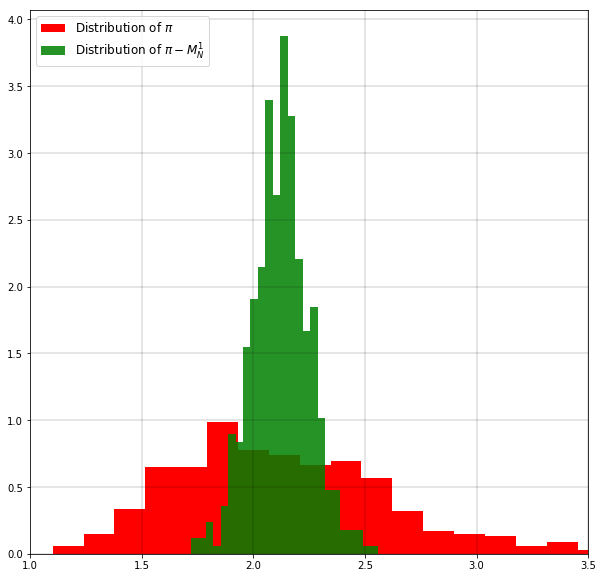
\includegraphics[width=0.4\textwidth]{pictures/gm_1d_test_exp.png}
\label{fig:subfig1}}
\qquad
\subfloat[Subfigure 2 list of figures text][d = 2]{
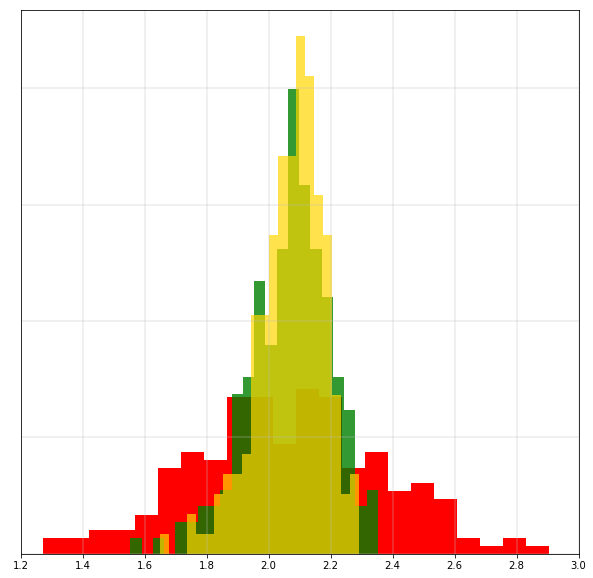
\includegraphics[width=0.4\textwidth]{pictures/gm_2d_test.png}
\label{fig:subfig2}}
\caption{\label{fig:1}Histograms for Gaussian mixture. (a) 1-dimensional GM model: histograms of estimators for target function $f(x) = e^x$ on test sample (200 independent trajectories obtained by ULA algorithm). \textit{Red} bins correspondent to ordinary weighted estimators $\pi^N_n(f)$, \textit{green} - variance-reduced estimators $\pi^N_{1,n}(f)$.\\ (b) 2-dimensional GM model: histograms of estimators for target function $f(x) = x_1^2 + x_2^2 - \cos(x_1)$, \textit{red} bins: $\pi^N_n(f)$, \textit{green}: $\pi^N_{1,n}(f)$, \textit{yellow}: $\pi^N_{2,n}(f)$.}
\end{figure}

\subsection{Gaussian mixtures}
 We consider a sample generated by ULA with $\pi$  given by the mixture of two Gaussian distributions  with equal weights:
\begin{eqnarray*}
\pi (x) = \frac{1}{2(2\pi)^{d/2}} \left( e ^{\frac{-| x-a|^2}{2}}  + e ^{\frac{-| x+a|^2}{2}} \right), \quad x \in\mathbb R^d
\end{eqnarray*}
where $a \in \mathbb{R}^d$ is a given vector. The function $U(x)$ and its gradient are given by
\begin{eqnarray*}
U(x) = \frac{1}{2} \|x - a\|_2^2 - \text{log}(1 + e^{-2x^\top a})
\end{eqnarray*}
and
\begin{eqnarray*}
\nabla U(x) = x-a +2a(1 + e^{2 x^\top a})^{-1},
\end{eqnarray*}
respectively.
\par
In our experiments we considered dimensions $d = 1$ and $d = 2$ and defined vector $a$ as $(\frac{1}{\sqrt{2d}}, \dots, \frac{1}{\sqrt{2d}})$ . For ULA  we used constant step sizes $\gamma_i = 0.2$ and $n=1000$. In order to approximate coefficients $a_{p,l,\mathbf{k}}(x),$ we generated $\NtrainPath = 500$ independent "training" trajectories and solved the least squares  problems \eqref{eq:06042018a1} with polynomial basis functions with maximum degree \(5\) and \(3\) for dimensions \(1\) and \(2\), respectively. More precisely we used the polynomials
\begin{eqnarray*}
\Psi^1 &=& \left\{1,x,x^2,x^3,x^4,x^5 \right\}, \text{ for } d = 1, \\
\Psi^2 &=& \left\{1,x_1,x_2,x_1 x_2,x_1^2,x_2^2, x_1^2 x_2,x_1x_2^2,x_1^3,x_2^3 \right\}, \text{ for }  d = 2.
\end{eqnarray*}
We fixed \(K = 1\) for \(d=1\) and \(K=2\) for \(d = 2\). To test our variance reduction algorithm, we generated $N_{\mathrm{test}} = 200$ independent paths and computed empirical variance of the new variance reduced estimator $\pi_{K,n}^N(f)$ of target functions $f(x) = e^x$ for $d = 1$ and $f(x) = x_1^2 + x_2^2 - \cos(x_1)$ for $d = 2$.
Figure ~\ref{fig:1} shows the histograms of weighted average estimator \(\pi_{n}^N(f)\) and variance reduced estimator \(\pi_{K,n}^N(f)\) computed on test sample. We have repeated the whole experiment \(5\) times and presented the results in Table ~\ref{table:gm}. Eventually, we can see that new estimator has considerably reduced variance in comparison with ordinary estimator.

\begin{table}[h]
\begin{tabular}{|l|lllll|}	
\hline
 &  &  &\(d = 1\)  &  &  \\ \hline
$\mathsf{Var}(\pi_n^N)$ &  0.28641 & 0.24557  &0.26398   &  0.27346 & 0.27845  \\
$\mathsf{Var}(\pi_{1,n}^N)$ & 0.02046 &  0.02068 & 0.02789 & 0.02218 &  0.01957\\ \hline
 &  &  &\(d = 2\)  &  &  \\ \hline
 $\mathsf{Var}(\pi_n^N)$     & 0.09238 & 0.10268 & 0.09458 &  0.09024 &  0.09312\\
 $\mathsf{Var}(\pi_{1,n}^N)$ & 0.01800 & 0.02156 & 0.01961 &  0.01288 &  0.01754\\
 $\mathsf{Var}(\pi_{2,n}^N)$ & 0.01155 & 0.01341 & 0.01097 &  0.00842 &  0.01018 \\ \hline
\end{tabular}
\caption{Gaussian Mixtures: Empirical variances of ordinary weighted and variance-reduced estimators on test sample.}
\label{table:gm}
\end{table}

\begin{figure}[h]
\begin{center}
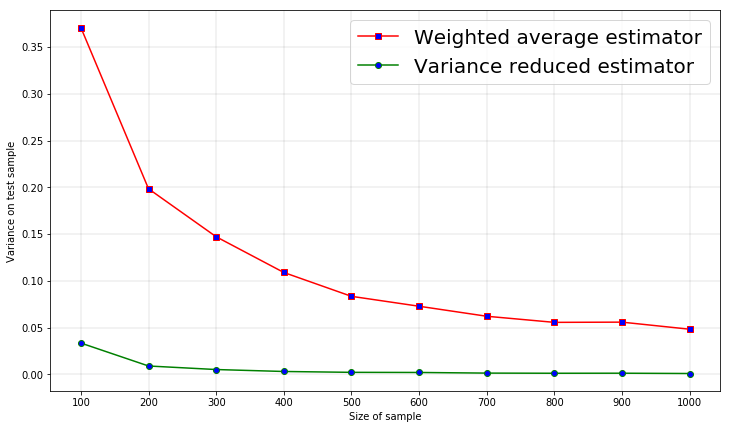
\includegraphics[height=0.5\textwidth]{pictures/comparison_gm.png}
\caption{\label{fig:comparison}1-dimensional GM model. Vertical axis is empirical variance on test sample, horizontal axis is the length of test trajectories obtained by ULA algorithm.Red traceplot correspondents to ordinary weighted estimator, green traseplot illustrates empirical variances of variance-reduced estimator for K=1.}
\end{center}
\end{figure}
In order to illustrate the dependence of variances of the proposed variance reduced estimator on  the  number of elements in trajectory,  we report in Figure ~\ref{fig:comparison}  the traceplots of the empirical variances versus $n$ for the case of the one-dimensional Gaussian mixture and K =1. One may observe that the sample size needed to achieve the "almost zero" variance  is much smaller for the variance reduced estimator \(\pi_{K,n}^N(f)\) than for the ordinary weighted average estimator \(\pi_{n}^N(f)\).



\begin{figure}[h]
\begin{center}
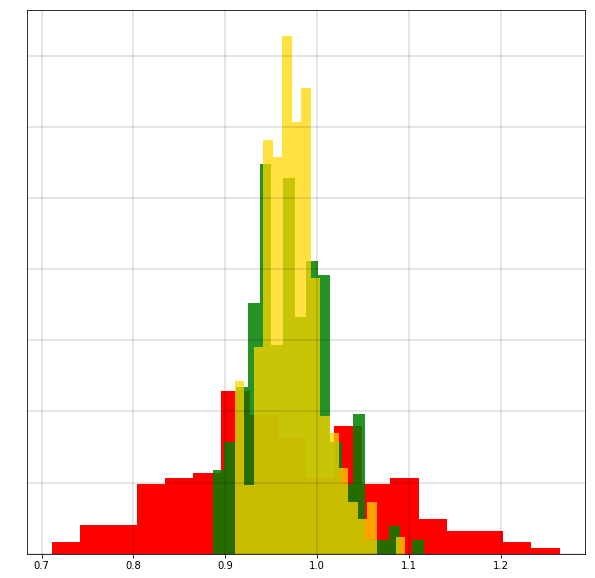
\includegraphics[height=0.5\textwidth]{pictures/blr_2d_test.png}
\caption{\label{fig:blr} Binary Logistic Regression: Histograms of estimators for target function $f(\theta) = 2 \theta_1^2 + 7 \theta_2^2$ on test sample. \textit{Red} bins correspondent to ordinary weighted estimators $\pi^N_n(f)$, \textit{green} - variance-reduced estimators $\pi^N_{1,n}(f)$and \textit{yellow} - $\pi^N_{2,n}(f)$.}
\end{center}
\end{figure}

\subsection{Binary Logistic regression}
Second experiment considers the problem of logistic regression, similar to that considered by Dalalyan \cite{dalalyan2017theoretical}. Suppose we have i.i.d. sample $\left\{ (\mathbf{X}_i, Y_i)\right\}$ for $ i =1, \dots , m$ with features $\mathbf{X}_i \in \mathbb{R}^p $ and binary labels $Y_i \in \left\{0,1 \right\}$. The binary logistic regression model defines the conditional distribution of $Y$ given $X$ by a logistic function
\begin{eqnarray*}
r(\theta, x) = \frac{e^{\theta^T x}}{1 + e^{\theta^T x}}
\end{eqnarray*}
where $\theta$ is parameter of model. In order to estimate $\theta$ according to given data, the Bayessian approach introduces prior distribution $\pi_0(\theta)$ and inferences the posterior density $\pi(\theta)$ using Bayes' rule. In case of Gaussian prior $\pi_0$ with zero mean and covariance matrix proportional to the inverse of the Gram matrix $\mathbf{\Sigma_X} = \frac{1}{n} \sum_{i=1}^m \mathbf{X}_i \mathbf{X}_i^T$, the posterior density takes the form
\begin{eqnarray*}
\pi(\theta) \propto \exp \left\{ -  \mathbf{Y}^T \mathbf{X \theta} - \sum_{i=1}^m \text{log} (1 + e^{-\mathbf{\theta}^T \mathbf{X}_i}) - \frac{\lambda}{2} \left\| \mathbf{\Sigma_X}^{1/2} \mathbf{\theta}\right\|_2^2 \right\}
\end{eqnarray*}
where $\mathbf{Y}$ defined as $(Y_1, \dots, Y_m)^T \in \left\{ 0,1\right\}$ and $\lambda > 0$ additional parameter specified by practitioner. Denote
\begin{eqnarray*}
U( \mathbf{\theta}) = \mathbf{Y}^T \mathbf{X \theta} + \sum_{i=1}^m \text{log} (1 + e^{-\mathbf{\theta}^T \mathbf{X}_i}) + \frac{\lambda}{2} \left\| \mathbf{\Sigma_X}^{1/2} \mathbf{\theta}\right\|_2^2
\end{eqnarray*}
\begin{eqnarray*}
\nabla U(\mathbf{\theta}) = \mathbf{X}^T \mathbf{Y} - \sum_{i=1}^m \frac{\mathbf{X}_i}{1 + e^{\mathbf{\theta}^T \mathbf{X}_i}} + \lambda \mathbf{\Sigma_X \theta}
\end{eqnarray*}

\begin{table}[h]
\begin{tabular}{|l|lllll|}	
\hline
 &  &  &\(d = 2\)  &  &  \\ \hline
$\operatorname{Var}(\pi_n^N)$    & 0.03727 &  0.02124 &  0.04769  & 0.01147  & 0.02974   \\
$\operatorname{Var}(\pi_{1,n}^N)$& 0.00269 &  0.00224 &  0.00306  & 0.00179  & 0.00196  \\
$\operatorname{Var}(\pi_{2,n}^N)$& 0.00182 &  0.00117 &  0.00213  & 0.00100  & 0.00107 \\ \hline
\end{tabular}
\caption{BLR: Empirical variance of ordinary weighted and variance-reduced estimators on test sample.}
\label{table:blr}
\end{table}

In our second experiment, we randomly generated $m$ independent samples as in paper \cite{dalalyan2017theoretical}, more precisely features $\mathbf{X}_i$ were generated from a Rademacher distribution and then normalized to have an norm equal to one. Each target variable $Y_i$ has been obtained from a Bernoulli distribution with parameter $r (\mathbf{\theta}_{\text{true}},\mathbf{x})$, where $\mathbf{\theta}_{\text{true}}$ is defined as $(1, \dots, 1)^T$. We fix $d = 2$ and generated $m = 50$ samples according Rademacher distribution. To construct trajectories of length $n = 500 $ we determined constant step size $\gamma_i = 0.02$ for ULA scheme. As in previous experiment we use polynomials approximations to explicitly compute $a_{p,l,k}$ and fixed $\NtrainPath = 300$, $N_{test} = 200$ and $K=2$. The target function defined as
\begin{eqnarray*}
f(\mathbf{\theta}) = 2 \theta_1^2 + 7 \theta_2^2
\end{eqnarray*}
Table ~\ref{table:blr} summarizes results of conventional weighted estimator and variance reduced estimator.



\section{Proofs}
\subsection{Proof of Theorem~\ref{th:mr}}
We start with introducing some notations.
For $m\in\mathbb N$, a smooth function
$h\colon\mathbb R^{d\times m}\to\mathbb R$
with arguments being denoted
$(y_1,\ldots,y_m)$, $y_i\in\mathbb R^d$, $i=1,\ldots,m$,
a multi-index $\mathbf k=(k_i)\in\mathbb N_0^d$,
and $j\in\{1,\ldots,m\}$,
we use the notation $\partial^{\mathbf k}_{y_j} h$ for the multiple derivative of $h$
with respect to the components of~$y_j$:
$$
\partial^{\mathbf k}_{y_j} h(y_1,\ldots,y_m)
:=\partial^{k_d}_{y_j^d}
\ldots
\partial^{k_1}_{y_j^1}
h(y_1,\ldots,z_m),
\quad y_j=(y_j^1,\ldots,y_j^d).
$$
In the particular case $m=1$ we can drop
the subscript $y_1$ in that notation.
For $l\le p$, we have the representation
\[
X_{p}=G_{p,l}(X_{l-1},\sqrt{\gamma_{l}}Z_{l},\ldots,\sqrt{\gamma_{p}}Z_{p}),
\]
where the function \(G_{p,l}:\) \(\mathbb{R}^{d\times(p-l+2)}\to \mathbb{R}^{d}\) is defined as
\begin{equation}
\label{eq:definition-G-p-l}
G_{p,l}(x,y_l,\ldots,y_p):=\Phi_{p}(\cdot,y_{p})\circ\Phi_{p-1}(\cdot,y_{p-1})\circ\ldots\circ\Phi_{l}(x,y_{l})
\end{equation}
with
\[
\Phi_{j}(x,y)=x-\gamma_{j}\mu(x)+y,
\quad x,y\in\mathbb R^d.
\]
As a consequence,
for a function $f\colon\mathbb R^d\to\mathbb R$
as in Section~\ref{sec:setup}, we have
$$
f\left(X_{p}\right) =f\circ G_{p,l}(X_{l-1},\sqrt{\gamma_{l}}Z_{l},\ldots,\sqrt{\gamma_{p}}Z_{p}).
$$
In what follows, for $\mathbf{k}\in\mathbb N_0^d$,
we use the shorthand notation
\begin{equation}
\label{eq:definition-differential-f-p}
\partial_{y_l}^{\mathbf k} f\left(X_{p}\right)
:=\partial_{y_l}^{\mathbf k} [f\circ G_{p,l}](X_{l-1},\sqrt{\gamma_{l}}Z_{l},\ldots,\sqrt{\gamma_{p}}Z_{p})
\end{equation}
whenever the function $f\circ G_{p,l}$ is smooth enough
(that is, $f$ and $\mu$ need to be smooth enough).
Finally, for a multi-index $\mathbf{k}=(k_i)\in\mathbb N_0^d$, we use the notation
\(\mathbf{k} ! :=k_1!\cdot\ldots\cdot k_d !\)

\begin{lem}\label{eq:a_repr}
Fix $l\le p$ and some \(\mathbf{k},\mathbf{k}'\in \mathbb{N}_0^d\) with \(\mathbf{k}'\le \mathbf{k}\) componentwise.  Then the following representation holds
$$
a_{p,l,\mathbf{k}}(X_{l-1})=\left(\gamma_{l}^{|\mathbf{k}'|}\frac{(\mathbf{k}-\mathbf{k}') !}{\mathbf{k}!}\right)^{1/2}
\mathsf E\left[\left.
\partial_{y_l}^{\mathbf{k}'}f(X_p)\mathbf{H}_{\mathbf{k}-\mathbf{k}'}(Z_l)\right|X_{l-1}\right].
$$
\end{lem}

\begin{proof}
Let $\boldsymbol{\varphi}(z)=\frac{1}{(2\pi)^{d/2}} \exp\{-|z|^2/2\}$,
$z\in\mathbb R^d$, denote the density of a $d$-dimensional
standard Gaussian random vector.
We first remark that, for the normalized Hermite polynomial $\mathbf H_{\mathbf k}$ on $\mathbb R^d$,
$\mathbf k\in\mathbb N_0^d$, it holds
$$
\mathbf{H}_{\mathbf{k}}(z)\boldsymbol{\varphi}(z)
=\frac{(-1)^{|\mathbf{k}|}}{\sqrt{\mathbf{k} !}} \partial^{\mathbf{k}} \boldsymbol{\varphi}(z).
$$
This enables to use the integration by parts in vector form as follows
(below $\prod_{j=l+1}^p:=1$ whenever $l=p$)
\begin{align*}
&a_{p,l,\mathbf k}(x)
 =
\int_{\mathbb R^d}\ldots\int_{\mathbb R^d}
f\circ G_{p,l}(x,\sqrt{\gamma_{l}}z_{l},\ldots,\sqrt{\gamma_{p}}z_{p})
\mathbf{H}_{\mathbf{k}}(z_{l})\boldsymbol{\varphi}(z_l)
\prod_{j=l+1}^p\boldsymbol{\varphi}(z_j)\, dz_{l}\ldots dz_{p}
\\
& =
\frac{1}{\sqrt{\mathbf k!}}
\int_{\mathbb R^d}\ldots\int_{\mathbb R^d}
f\circ G_{p,l}(x,\sqrt{\gamma_{l}}z_{l},\ldots,\sqrt{\gamma_{p}}z_{p})
(-1)^{|\mathbf{k}|}\partial^{\mathbf{k}} \boldsymbol{\varphi}(z_l)
\prod_{j=l+1}^p\boldsymbol{\varphi}(z_j)\, dz_{l}\ldots dz_{p}
\\
& =
\gamma_l^{|\mathbf k'|/2}\frac{1}{\sqrt{\mathbf k!}}
\int_{\mathbb R^d}\ldots\int_{\mathbb R^d}
\partial_{y_l}^{\mathbf k'}[f\circ G_{p,l}](x,\sqrt{\gamma_{l}}z_{l},\ldots,\sqrt{\gamma_{p}}z_{p})
\\
&\hspace{1em}\times
(-1)^{|\mathbf{k}-\mathbf k'|}\partial^{\mathbf{k}-\mathbf k'} \boldsymbol{\varphi}(z_l)
\prod_{j=l+1}^p\boldsymbol{\varphi}(z_j)\, dz_{l}\ldots dz_{p}
\\
& =
\gamma_l^{|\mathbf k'|/2}\frac{\sqrt{(\mathbf k-\mathbf k')!}}{\sqrt{\mathbf k!}}
\int_{\mathbb R^d}\ldots\int_{\mathbb R^d}
\partial_{y_l}^{\mathbf k'}[f\circ G_{p,l}](x,\sqrt{\gamma_{l}}z_{l},\ldots,\sqrt{\gamma_{p}}z_{p})
\\
&\hspace{1em}\times
\mathbf{H}_{\mathbf{k}-\mathbf k'}(z_{l})\boldsymbol{\varphi}(z_l)
\prod_{j=l+1}^p\boldsymbol{\varphi}(z_j)\, dz_{l}\ldots dz_{p}
\\
 & =\gamma_{l}^{|\mathbf{k}'|/2}\frac{\sqrt{(\mathbf{k}-\mathbf{k}')!}}{\sqrt{\mathbf{k}!}}\mathsf{E}\left[\partial_{y_{l}}^{\mathbf{k}'}[f\circ G_{p,l}](x,\sqrt{\gamma_{l}}Z_{l},\ldots,\sqrt{\gamma_{p}}Z_{p})\mathbf{H}_{\mathbf{k}-\mathbf{k}'}(Z_{l})\right].
\end{align*}
The last expression yields the result.
\end{proof}

For multi-indices $\mathbf k,\mathbf k'\in\mathbb N_0^d$
with $\mathbf k'\le\mathbf k$ componentwise
and $\mathbf k'\ne\mathbf k$,
we get applying first Lemma~\ref{eq:a_repr}
\begin{equation*}
\begin{split}
\bar a_{l,\mathbf{k}}(X_{l-1})
&=\left(\gamma_{l}^{|\mathbf{k}'|}\frac{(\mathbf{k}-\mathbf{k}')!}{\mathbf{k}!}\right)^{1/2}
\,\sum_{p=l}^{N+n}\omega_{p,n}^N
\mathsf E\left[\left.
\partial_{y_l}^{\mathbf{k}'}f(X_p)\mathbf{H}_{\mathbf{k}-\mathbf{k}'}(Z_l)\right|X_{l-1}\right]\\
&=\left(\gamma_{l}^{|\mathbf{k}'|}\frac{(\mathbf{k}-\mathbf{k}')!}{\mathbf{k}!}\right)^{1/2}
\,\sum_{p=l}^{N+n}\omega_{p,n}^N
\mathsf E\left[\left.
\left(
\partial_{y_l}^{\mathbf{k}'}f(X_p)-\mathsf E\left[\partial_{y_l}^{\mathbf{k}'}f(X_p)|X_{l-1}\right]
\right)
\mathbf{H}_{\mathbf{k}-\mathbf{k}'}(Z_l)\right|X_{l-1}\right].
\end{split}
\end{equation*}

Assume that $\mu$ and $f$ are $K\times d$ times continuously differentiable.
Then, given $\mathbf k\in\mathbb N_0^d$,
by taking $\mathbf k'= \mathbf k'(\mathbf k)
=(K1_{\{k_1>K\}},\ldots,K1_{\{k_d>K\}})$,
for each $l\in\{N+1,\ldots,N+n\}$, we get
\begin{align}
\label{eq:sum_abar}
\sum_{\mathbf{k}\colon\|\mathbf{k}\|\geq K+1}\left[\bar{a}_{l,\mathbf{k}}^{2}(X_{l-1})|\mathcal{G}_{N}\right] & =\sum_{\mathbf{k}\colon\|\mathbf{k}\|\geq K+1}\left(\gamma_{l}^{|\mathbf{k}'|}\frac{(\mathbf{k}-\mathbf{k}')!}{\mathbf{k}!}\right)Q(\mathbf{k}',\mathbf{k}-\mathbf{k}')\\
\nonumber
 & =\sum_{I\subseteq\{1,\ldots,d\},\, I\neq \emptyset}\gamma_{l}^{|I|K}\sum_{\mathbf{m}_{I}\in\mathbb{N}_{I}^{d}}\frac{\mathbf{m}_{I}!}{\left(\mathbf{m}_{I}+\mathbf{K}_{I}\right)!}
 \\
 \nonumber
 & \hspace{1em}\times\sum_{\mathbf{m}_{I^c}\in \mathbb{N}^d_{0,I^c},\,\|\mathbf{m}_{I^c}\|\leq K}Q(\mathbf{\mathbf{K}}_{I},\mathbf{m}_{I}+\mathbf{m}_{I^c}),
\end{align}
where for any two multi-indices \(\mathbf{r},\) \(\mathbf{q}\) from \(\mathbb{N}_0^d\)
\begin{eqnarray*}
Q(\mathbf{r},\mathbf{q})=\mathsf{E}\left\{
\left(\mathsf{E}\left[\sum_{p=l}^{N+n}\omega_{p,n}^{N}\left(\partial_{y_{l}}^{\mathbf r}f\left(X_{p}\right)-\mathsf{E}\left[\partial_{y_{l}}^{\mathbf r}f\left(X_{p}\right)|X_{l-1}\right]\right)\mathbf{H}_{\mathbf{q}}(Z_{l})\Big|X_{l-1}\right]\right)^{2}
\Bigg|\mathcal G_N \right\}.
\end{eqnarray*}
In \eqref{eq:sum_abar} the first sum runs over all nonempty subsets $I$ of the set $\{1,\ldots,d\}.$
For any subset $I,$ $\mathbb{N}_{I}^{d}$ stands for a set
of multi-indices $\mathbf{m}_{I}$ with elements $m_{i}=0,$ $i\not\in I,$
and $m_{i}\in\mathbb{N},$  $i\in I.$ Moreover, \(I^c=\{1,\ldots,d\}\setminus I\) and \(\mathbb{N}^d_{0,I^c}\) stands for a set
of multi-indices $\mathbf{m}_{I^c}$ with elements $m_{i}=0,$ $i\in I,$
and $m_{i}\in\mathbb{N}_0,$  $i\not\in I.$ Finally, the multi-index \(\mathbf{K}_I\) is defined as $\mathbf{\mathbf{K}}_{I}=(K1_{\{1\in I\}},\ldots,K1_{\{d\in I\}}).$
Applying the estimate
\begin{eqnarray*}
\frac{\mathbf{m}_{I}!}{\left(\mathbf{m}_{I}+\mathbf{K}_{I}\right)!}\leq (1/2)^{|I| K},
\end{eqnarray*}
we get
\begin{eqnarray*}
\sum_{\mathbf{k}\colon\|\mathbf{k}\|\geq K+1}\left[\bar{a}_{l,\mathbf{k}}^{2}(X_{l-1})|\mathcal{G}_{N}\right]&\leq &
\sum_{I\subseteq\{1,\ldots,d\},\, I\neq \emptyset} (\gamma_{l}/2)^{|I|K}
\\
&& \times\sum_{\mathbf{m}_{I}\in\mathbb{N}_{I}^{d}} \sum_{\mathbf{m}_{I^c}\in \mathbb{N}^d_{0,I^c},\,\|\mathbf{m}_{I^c}\|\leq K} Q(\mathbf{\mathbf{K}}_{I},\mathbf{m}_{I}+\mathbf{m}_{I^c})
\\
&\leq &
\sum_{I\subseteq\{1,\ldots,d\},\, I\neq \emptyset} (\gamma_{l}/2)^{|I|K} \sum_{\mathbf{m}\in\mathbb{N}_0^{d}} Q(\mathbf{\mathbf{K}}_{I},\mathbf{m}).
\end{eqnarray*}
Now using the consequence
$\sum_{\mathbf{m}\in \mathbb{N}^d_0} \langle\xi,\mathbf{H}_\mathbf{m}(Z_l)\rangle^2\le\langle\xi,\xi\rangle$
of Parseval's identity
(the latter is used conditionally on $X_{l-1}$
%equivalently, on $\mathcal G_{l-1}$,
which is possible because the system
$\{\mathbf{H}_\mathbf{m}(Z_l)\}_{m\in \mathbb{N}^d_0}$
is orthonormal conditionally on $X_{l-1}$),
%and the tower property $\mathsf E[\mathsf E(\cdot|\mathcal G_{l-1})|\mathcal G_N]=\mathsf E[\cdot|\mathcal G_N]$
we derive
\begin{eqnarray*}
\sum_{\mathbf{k}\colon\|\mathbf{k}\|\geq K+1}\left[\bar{a}_{l,\mathbf{k}}^{2}(X_{l-1})|\mathcal{G}_{N}\right]
&\leq & \sum_{I\subseteq\{1,\ldots,d\},\, I\neq \emptyset}
\left(\frac{\gamma_{l}}{2}\right)^{|I|K}
\\
&& \times\mathsf E\left[
\mathsf{Var}\left(\sum_{p=l}^{N+n}\omega_{p,n}^{N}\partial_{y_{l}}^{\mathbf{K}_I}f\left(X_{p}\right)
\Big|X_{l-1}\right)
\Bigg|\mathcal G_N\right]
\\
&=& \frac{1}{\Gamma^2_{N+2,N+n+1}}\sum_{I\subseteq\{1,\ldots,d\},\, I\neq \emptyset}
\left(\frac{\gamma_{l}}{2}\right)^{|I|K}
R_{l,n,N}^{I,K}
\end{eqnarray*}
with
\begin{eqnarray*}
R_{l,n,N}^{I,K}=\mathsf E\left[
\mathsf{Var}\left(\sum_{p=l}^{N+n}\gamma_{p+1}\partial_{y_{l}}^{\mathbf{K}_I}f\left(X_{p}\right)
\Big|X_{l-1}\right)
\Bigg|\mathcal G_N\right].
\end{eqnarray*}
As a result
\begin{eqnarray*}
\mathsf{Var}\left[\left.\pi_{K,n}^{N}(f)\right|\mathcal G_N\right]\leq \frac{1}{\Gamma^2_{N+2,N+n+1}}\sum_{l=N+1}^{N+n}\sum_{I\subseteq\{1,\ldots,d\},\, I\neq \emptyset}
\left(\frac{\gamma_{l}}{2}\right)^{|I|K}
R_{l,n,N}^{I,K}.
\end{eqnarray*}
Next result we show that under the conditions  of Theorem~\ref{th:mr}, the quantity \(R_{l,n,N}^{I,K}\) is uniformly bounded in \(l,n,N,I.\) First we need to prove several auxiliary results.
\begin{lem}\label{lem:06062018a1}
Let $(x_p)_{p\in\mathbb N_0}$
and $(\epsilon_p)_{p\in\mathbb N}$
be sequences of nonnegative real numbers
satisfying $x_0=\ol C_0$ and
\begin{align}
0&\le x_p\le\alpha_p x_{p-1}+\gamma_p \epsilon_p,\quad p\in\mathbb N,
\label{eq:06062018a1}\\
0&\le\epsilon_p\le\ol C_1\prod_{k=1}^p \alpha_k^2,\quad p\in\mathbb N,
\label{eq:06062018a2}
\end{align}
where $\alpha_p,\gamma_p\in(0,1)$, $p\in\mathbb N$,
and $\ol C_0,\ol C_1$ are some nonnegative constants. Assume
\begin{equation}\label{eq:06062018a3}
\sum_{r=1}^\infty\gamma_r \prod_{k=1}^r \alpha_k\le\ol C_2
\end{equation}
for some constant $\ol C_2$. Then
$$
x_p\le(\ol C_0+\ol C_1\ol C_2)\prod_{k=1}^p \alpha_k,\quad p\in\mathbb N.
$$
\end{lem}

\begin{proof}
Applying~\eqref{eq:06062018a1} recursively, we get
$$
x_p\le\ol C_0\prod_{k=1}^p \alpha_k
+\sum_{r=1}^p \gamma_r\epsilon_r
\prod_{k=r+1}^p \alpha_k,
$$
where we use the convention $\prod_{k=p+1}^p:=1$.
Substituting estimate~\eqref{eq:06062018a2}
into the right-hand side, we obtain
$$
x_p\le\left(\ol C_0+\ol C_1
\sum_{r=1}^p \gamma_r \prod_{k=1}^r \alpha_k
\right)
\prod_{k=1}^p \alpha_k,
$$
which, together with~\eqref{eq:06062018a3}, completes the proof.
\end{proof}

In what follows, we use the notation
\begin{equation}
\label{eq:definition-alpha}
\alpha_k=1-\gamma_k b_\mu,\quad k\in\mathbb N.
\end{equation}

\begin{remark}\label{rem:10062018a1}
Notice that, under~\eqref{eq:17042018a1},
not only~\eqref{eq:06062018a3} but also
\begin{equation}\label{eq:10062018a1}
\sum_{r=j}^\infty\gamma_r \prod_{k=j}^r \alpha_k\le\ol C_2
\end{equation}
is satisfied with the same constant~$\ol C_2$
(which is $C$ of~\eqref{eq:17042018a1})
simultaneously for all $j\in\mathbb N$.
Below this will allow us to apply
Lemma~\ref{lem:06062018a1}
to bound double indexed sequences
$(x_{j,p})_{j\ge1,p\ge j}$
satisfying
$$
0\le x_{j,p}\le\alpha_p x_{j,p-1}+\gamma_p \epsilon_{j,p},\quad p\ge j+1,
$$
with suitable $(\epsilon_{j,p})_{j\ge1,p\ge j+1}$
and the constant $\ol C_2$ in~\eqref{eq:10062018a1}
being independent of~$j$.
\end{remark}

\begin{lem}\label{lem:06062018a2}
Under assumptions of Theorem~\ref{th:mr},
for all natural $r\le K$ and $l\le p$, there exist constants $C_r$ (not depending on $l$ and $p$) such that
\begin{equation}
\label{eq:08062018b2}
\left|\partial_{y_l}^r X_p \right| \le C_r\prod_{k=l+1}^p \alpha_k \,,
\end{equation}
where $\partial_{y_l}^r X_p$ is defined in \eqref{eq:definition-differential-f-p}. Moreover, we can choose $C_1=1$.
\end{lem}
\begin{proof}
The proof is along the same lines as Lemma~\ref{lem:06062018a3}.
\end{proof}
\begin{lem}\label{lem:06062018a3}
Under assumptions of Theorem~\ref{th:mr},
for all natural $r\le K$, $j\ge l$ and $p>j$, we have
\begin{equation}\label{eq:08062018b3}
\left|\partial_{y_j} \partial_{y_l}^r X_p\right|
\le c_r\prod_{k=l+1}^p \alpha_k
\end{equation}
with some constants $c_r$
not depending on $j$, $l$ and $p$,
while, for $p\le j$, it holds
$\partial_{y_{j}}\partial_{y_{l}}^{r}X_{p}=0$.
\end{lem}

\begin{proof}
The last statement is straightforward.
We fix natural numbers $j\ge l$ and prove~\eqref{eq:08062018b3}
for all $p>j$ by induction in~$r$.
First, for $p>j$, we write
$$
\partial_{y_{l}}X_{p}
=\left[1-\gamma_{p}\mu'(X_{p-1})\right]\partial_{y_{l}}X_{p-1}
$$
and differentiate this identity with respect to~$y_j$
$$
\partial_{y_{j}}\partial_{y_{l}}X_{p}
=\left[1-\gamma_{p}\mu'(X_{p-1})\right]\partial_{y_{j}}\partial_{y_{l}}X_{p-1}-\gamma_{p}\mu''(X_{p-1})\partial_{y_{j}}X_{p-1}\partial_{y_{l}}X_{p-1}.
$$
By Lemma~\ref{lem:06062018a2}, we have
\begin{align*}
|\partial_{y_{j}}\partial_{y_{l}}X_{p}|
&\le\alpha_p|\partial_{y_{j}}\partial_{y_{l}}X_{p-1}|
+\gamma_{p}
B_\mu
\prod_{k=l+1}^{p-1}\alpha_k
\prod_{k=j+1}^{p-1}\alpha_k\\
&\le\alpha_p|\partial_{y_{j}}\partial_{y_{l}}X_{p-1}|
+\gamma_{p}
\const
\prod_{k=l+1}^{j}\alpha_k
\prod_{k=j+1}^{p}\alpha_k^2,
\quad p\ge j+1,
\end{align*}
with a suitable constant
(we can take, e.g., $\const=\frac{B_\mu}{(1-\gamma_1 b_\mu)^2}$).
By Lemma~\ref{lem:06062018a1}
together with Remark~\ref{rem:10062018a1} applied
to bound $|\partial_{y_{j}}\partial_{y_{l}}X_{p}|$
for $p\ge j+1$
(notice that $\partial_{y_j}\partial_{y_l}X_j=0$, that is,
$\ol C_0$ in Lemma~\ref{lem:06062018a1} is zero,
while $\ol C_1$ in Lemma~\ref{lem:06062018a1}
has the form $\const\prod_{k=l+1}^j \alpha_k$),
we obtain~\eqref{eq:08062018b3} for $r=1$.

The induction hypothesis is now that the inequality
\begin{equation}\label{eq:induc-derive}
\left|\partial_{y_{j}}\partial_{y_{l}}^{k}X_{p}\right|
\leq c_{k}\prod_{s=l+1}^{p}\alpha_{s}
\end{equation}
holds for all natural $k<r\;(\le K)$ and $p>j$.
We need to show~\eqref{eq:induc-derive} for $k=r$.
Fa\`a di Bruno's formula implies for $2\le r\le K$ and $p>l$
\begin{align}
\partial_{y_{l}}^{r}X_{p}
&=\left[1-\gamma_{p}\mu'(X_{p-1})\right]\partial_{y_{l}}^{r}X_{p-1}
\label{eq:08062018a1}\\
&\hspace{1em}-\gamma_{p}\sum\frac{r!}{m_{1}!\ldots m_{r-1}!\,}\mu^{(m_{1}+\ldots+m_{r-1})}(X_{p-1})\prod_{k=1}^{r-1}\left(\frac{\partial_{y_{l}}^{k}X_{p-1}}{k!}\right)^{m_{k}},
\notag
\end{align}
where the sum is taken over all $(r-1)$-tuples of nonnegative integers
$(m_{1},\ldots,m_{r-1})$ satisfying the constraint
\begin{equation}\label{eq:09062018a1}
1\cdot m_{1}+2\cdot m_{2}+\ldots+(r-1)\cdot m_{r-1}=r.
\end{equation}
Notice that we work with $(r-1)$-tuples
rather than with $r$-tuples
because the term containing
$\partial_{y_l}^r X_{p-1}$
on the right-hand side of~\eqref{eq:08062018a1}
is listed separately.
For $p>j$, we then have
\begin{align}
&\partial_{y_{j}}\partial_{y_{l}}^{r}X_{p}
=\left[1-\gamma_{p}\mu'(X_{p-1})\right]\partial_{y_{j}}\partial_{y_{l}}^{r}X_{p-1}-\gamma_{p}\mu''(X_{p-1})\partial_{y_{l}}^{r}X_{p-1}\partial_{y_{j}}X_{p-1}
\label{eq:09062018a2}\\
&\hspace{1em}-\gamma_{p}\sum\frac{r!}{m_{1}!\ldots m_{r-1}!\,}\mu^{(m_{1}+\ldots+m_{r-1}+1)}(X_{p-1})\partial_{y_{j}}X_{p-1}\prod_{k=1}^{r-1}\left(\frac{\partial_{y_{l}}^{k}X_{p-1}}{k!}\right)^{m_{k}}
\notag\\
&\hspace{1em}-\gamma_{p}\sum\frac{r!}{m_{1}!\ldots m_{r-1}!\,}\mu^{(m_{1}+\ldots+m_{r-1})}(X_{p-1})\partial_{y_{j}}\left[\prod_{k=1}^{r-1}\left(\frac{\partial_{y_{l}}^{k}X_{p-1}}{k!}\right)^{m_{k}}\right]
\notag\\
&\hspace{1em} =\left[1-\gamma_{p}\mu'(X_{p-1})\right]\partial_{y_{j}}\partial_{y_{l}}^{r}X_{p-1}+\gamma_{p}\epsilon_{l,j,p},
\notag
\end{align}
where the last equality defines the quantity $\epsilon_{l,j,p}$.
Furthermore,
\[
\partial_{y_{j}}\left[\prod_{k=1}^{r-1}\left(\frac{\partial_{y_{l}}^{k}X_{p-1}}{k!}\right)^{m_{k}}\right]=\sum_{s=1}^{r-1}\frac{m_{s}}{s!}\left(\frac{\partial_{y_{l}}^{s}X_{p-1}}{s!}\right)^{m_{s}-1}\partial_{y_{j}}\partial_{y_{l}}^{s}X_{p-1}\prod_{k\le r-1,\,k\neq s}\left(\frac{\partial_{y_{l}}^{k}X_{p-1}}{k!}\right)^{m_{k}}.
\]
Using Lemma~\ref{lem:06062018a2},
induction hypothesis~\eqref{eq:induc-derive}
and the fact that $m_{1}+\ldots+m_{r-1}\ge2$
for $(r-1)$-tuples of nonnegative integers
satisfying~\eqref{eq:09062018a1},
we can bound $|\epsilon_{l,j,p}|$ as follows
\begin{align*}
&\left|\epsilon_{l,j,p}\right|  \leq  B_{\mu}C_{r}\prod_{k=l+1}^{p-1}\alpha_{k}\prod_{k=j+1}^{p-1}\alpha_{k}+B_{\mu}\sum\frac{r!}{m_{1}!\ldots m_{r-1}!\,}\left[\prod_{k=j+1}^{p-1}\alpha_{k}\right]\prod_{s=1}^{r-1}\left(\frac{C_{s}\prod_{k=l+1}^{p-1}\alpha_{k}}{s!}\right)^{m_{s}}\\
&+B_{\mu}\sum\frac{r!}{m_{1}!\ldots m_{r-1}!\,}\sum_{t=1}^{r-1}\frac{m_t}{t!}\left(\frac{C_{t}\prod_{k=l+1}^{p-1}\alpha_{k}}{t!}\right)^{m_{t}-1}
c_t\left[\prod_{k=l+1}^{p-1}\alpha_{k}\right]\prod_{s\le r-1,\,s\neq t}\left(\frac{C_{s}\prod_{k=l+1}^{p-1}\alpha_{k}}{s!}\right)^{m_{s}}\\
& \leq \const\prod_{k=l+1}^{j}\alpha_{k}\prod_{k=j+1}^{p}\alpha_{k}^{2}
\end{align*}
with some constant ``$\const$'',
which is, in fact, $\frac1{(1-\gamma_1 b_\mu)^2}$ times
the expression involving
$B_\mu,r,C_1,\ldots,C_r,c_1,\ldots,c_{r-1}$.
Thus, \eqref{eq:09062018a2} now implies
$$
|\partial_{y_{j}}\partial_{y_{l}}^{r}X_{p}|
\le\alpha_p|\partial_{y_{j}}\partial_{y_{l}}^{r}X_{p-1}|
+\gamma_p \const\prod_{k=l+1}^{j}\alpha_{k}\prod_{k=j+1}^{p}\alpha_{k}^{2},
\quad p\ge j+1.
$$
We can again apply Lemma~\ref{lem:06062018a1}
and Remark~\ref{rem:10062018a1}
to bound $|\partial_{y_{j}}\partial_{y_{l}}^r X_{p}|$
for $p\ge j+1$
(notice that $\partial_{y_j}\partial_{y_l}^r X_j=0$, that is,
$\ol C_0$ in Lemma~\ref{lem:06062018a1} is zero,
while $\ol C_1$ in Lemma~\ref{lem:06062018a1}
has the form $\const\prod_{k=l+1}^j \alpha_k$),
and we obtain~\eqref{eq:induc-derive} for $k=r$.
This concludes the proof.
\end{proof}

\begin{lem}
\label{lem:var_poincare}
Under assumptions of Theorem~\ref{th:mr},
for all natural $l\le q$, it holds
$$
\mathsf{Var}\left[\sum_{p=l}^{q}\gamma_{p+1}\partial_{y_{l}}^{K}f\left(X_{p}\right)\Big|X_{l-1}\right]\le B_K\quad\text{a.s.},
$$
where $B_K$ is a deterministic bound that does not depend on $l$ and~$q$.
\end{lem}

\begin{proof}
The expression
$\sum_{p=l}^q \gamma_{p+1} \partial_{y_l}^K f(X_p)$
can be viewed as a deterministic function of
$X_{l-1},Z_l,Z_{l+1},\ldots,Z_q$
$$
\sum_{p=l}^q \gamma_{p+1} \partial_{y_l}^K f(X_p)
=F(X_{l-1},Z_l,Z_{l+1},\ldots,Z_q).
$$
By the (conditional) Gaussian Poincar\'e inequality,
we have
$$
\mathsf{Var}\left[\sum_{p=l}^{q}\gamma_{p+1}\partial_{y_{l}}^{K}f\left(X_{p}\right)\Big|X_{l-1}\right]
\le\mathsf E\left[\left.
\|\nabla_Z F(X_{l-1},Z_l,Z_{l+1},\ldots,Z_q)\|^2
\right|X_{l-1}\right],
$$
where $\nabla_Z F=(\partial_{Z_l} F,\ldots,\partial_{Z_q} F)$,
and $\|\cdot\|$ denotes the Euclidean norm.
Notice that
$$
\partial_{Z_j} F=\sqrt{\gamma_j}\,\partial_{y_j} F,
$$
hence,
$$
\mathsf{Var}\left[\sum_{p=l}^{q}\gamma_{p+1}\partial_{y_{l}}^{K}f\left(X_{p}\right)\Big|X_{l-1}\right]\leq\sum_{j=l}^{q}\gamma_{j}\mathsf{E}\left[\left(\sum_{p=l}^{q}\gamma_{p+1}\partial_{y_{j}}\partial_{y_{l}}^{K}f\left(X_{p}\right)\right)^{2}\Big|X_{l-1}\right].
$$
It is straightforward to check that
$\partial_{y_j}\partial_{y_l}^K f(X_p)=0$
whenever $p<j$. Therefore, we get
\begin{equation}\label{eq:10062018a2}
\mathsf{Var}\left[\sum_{p=l}^{q}\gamma_{p+1}\partial_{y_{l}}^{K}f\left(X_{p}\right)\Big|X_{l-1}\right]\leq\sum_{j=l}^{q}\gamma_{j}\mathsf{E}\left[\left(\sum_{p=j}^{q}\gamma_{p+1}\partial_{y_{j}}\partial_{y_{l}}^{K}f\left(X_{p}\right)\right)^{2}\Big|X_{l-1}\right].
\end{equation}
Now fix $p$ and $j$, $p\ge j$, in $\{l,\ldots,q\}$.
By Fa\`a di Bruno's formula
\[
\partial_{y_{l}}^{K}f\left(X_{p}\right)=\sum\frac{K!}{m_{1}!\ldots m_{K}!}f^{(m_{1}+\ldots+m_{K})}(X_{p})\prod_{k=1}^{K}\left(\frac{\partial_{y_{l}}^{k}X_{p}}{k!}\right)^{m_{k}},
\]
where the sum is taken over all $K$-tuples of nonnegative integers
$(m_1,\ldots,m_K)$ satisfying
$$
1\cdot m_{1}+2\cdot m_{2}+\ldots+K\cdot m_{K}=K.
$$
Then
\begin{align*}
&\partial_{y_{j}}\partial_{y_{l}}^{K}f\left(X_{p}\right)
=\sum\frac{K!}{m_{1}!\ldots m_{K}!}f^{(m_{1}+\ldots+m_{K}+1)}(X_{p})\left[\partial_{y_{j}}X_{p}\right]\prod_{k=1}^{K}\left(\frac{\partial_{y_{l}}^{k}X_{p}}{k!}\right)^{m_{k}} \\
&+\sum\frac{K!}{m_{1}!\ldots m_{K}!}f^{(m_{1}+\ldots+m_{K})}(X_{p})
\sum_{s=1}^{K}\frac{m_{s}}{s!}
\left(\frac{\partial_{y_{l}}^{s}X_{p}}{s!}\right)^{m_{s}-1}
\left[\partial_{y_{j}}\partial_{y_{l}}^{s}X_{p}\right]
\prod_{k\le K,\,k\neq s}\left(\frac{\partial_{y_{l}}^{k}X_{p}}{k!}\right)^{m_{k}}.
\end{align*}
Using the bounds of
Lemmas \ref{lem:06062018a2} and~\ref{lem:06062018a3},
we obtain
\[
\left|\partial_{y_{j}}\partial_{y_{l}}^{K}f\left(X_{p}\right)\right|
\leq A_{K}\prod_{k=l+1}^{p}\alpha_{k}
\]
with a suitable constant $A_{K}$.
Substituting this in~\eqref{eq:10062018a2},
we proceed as follows
\begin{align*}
\mathsf{Var}\left[\sum_{p=l}^{q}\gamma_{p+1}\partial_{y_{l}}^{K}f\left(X_{p}\right)\Big|X_{l-1}\right]
&\le
A_{K}^{2}\sum_{j=l}^{q}\gamma_{j}
\left(\sum_{p=j}^{q}\gamma_{p+1}\prod_{k=l+1}^{p}\alpha_{k}\right)^{2}
\\
&\le
\frac{A_{K}^{2}}{(1-\gamma_1 b_\mu)^2}
\sum_{j=l}^{q} \gamma_{j}
\left(
\sum_{p=j+1}^{q+1} \gamma_{p} \prod_{k=l+1}^{p} \alpha_{k}
\right)^{2}
\\
&=
\frac{A_{K}^{2}}{(1-\gamma_1 b_\mu)^2}
\sum_{j=l}^{q} \gamma_{j}
\prod_{k=l+1}^{j} \alpha_{k}^2
\left(
\sum_{p=j+1}^{q+1} \gamma_{p} \prod_{k=j+1}^{p} \alpha_{k}
\right)^{2}
\\
&\le
\frac{A_{K}^{2}}{(1-\gamma_1 b_\mu)^3}
\sum_{j=l}^{q} \gamma_{j}
\prod_{k=l}^{j} \alpha_{k}
\left(
\sum_{p=j+1}^{q+1} \gamma_{p} \prod_{k=j+1}^{p} \alpha_{k}
\right)^{2}
\\
&\le
\frac{A_{K}^{2}}{(1-\gamma_1 b_\mu)^3}C^3=B_K,
\end{align*}
where $C$ is the bound from~\eqref{eq:17042018a1}.
The proof is completed.
\end{proof}

\subsection{Proof of Lemma~\ref{a_decay}}

We have for any \(\mathbf{k}\neq \mathbf{0}\)
\begin{eqnarray*}
a_{p,l,\mathbf{k}}(x)=\mathsf{E}\left[\mathbf{H}_\mathbf{k}\left(Z_l\right)[Q_{p,l}\left(\Phi_l(x,Z_l)\right)-Q_{p,l}\left(\Phi_l(x,0)\right)]\right].
\end{eqnarray*}
Hence
\begin{eqnarray*}
\|a_{p,l,\mathbf{k}}\|_{\infty}\leq \sqrt{\gamma_l}\|Q'_{p,l}\|_{\infty}.
\end{eqnarray*}
Since \(f,\mu\in C^1(\mathbb{R}),\)  we have
\begin{eqnarray*}
Q'_{p,l}(x)=\mathsf{E}\left[(1-\gamma_{l+1}\mu'(x))Q'_{p,l+1}(x-\gamma_{l+1}\mu(x)+\sqrt{\gamma_{l+1}}\xi)\right].
\end{eqnarray*}
Hence
\begin{eqnarray*}
\|Q'_{p,l}\|_\infty\leq (1-b_{\mu}\gamma_{l+1})\|Q'_{p,l+1}\|_\infty
\end{eqnarray*}
and
\begin{eqnarray*}
\|Q'_{p,l}\|_\infty&\leq & \|f'\|_\infty\prod_{r=l+1}^p (1-b_{\mu}\gamma_{r})
\\
&\leq & \|f'\|_\infty\exp\left(-b_{\mu}\sum_{r=l+1}^p \gamma_{r}  \right).
\end{eqnarray*}
As a result
\begin{eqnarray*}
\|a_{p,l,\mathbf{k}}\|_{\infty}\leq \sqrt{\gamma_l}\, \|f'\|_\infty\exp\left(-b_{\mu}\sum_{r=l+1}^p \gamma_{r}  \right).
\end{eqnarray*}



\bibliographystyle{abbrv}
\bibliography{refs-1}
\end{document} 